\chapter{Light dark matter}\label{chap:1}

Most of the matter in the universe has been detected only through its gravity. It shapes galaxies and the cosmic microwave background and outweighs the atoms we know five to one, yet decades of searches for a heavy particle that recoils off a nucleus have found nothing. Those null results have shifted attention to lighter particles, below a GeV, which carry too little momentum to move a nucleus measurably but enough energy to lift an electron across a band gap or to set a crystal lattice vibrating. Detecting them turns a dark-matter search into a problem in condensed-matter physics: the target is no longer a collection of free nuclei but a solid, with all of its electronic and vibrational structure. The rate at which a detector registers dark-matter events sets what it can see, and that rate factorizes into a dark-matter part, the halo and the coupling, and the response of the solid.

\section{The master equation of direct detection}\label{sec:1.1}

A dark-matter detector counts events. Each one is a small burst of electron--hole pairs, phonons, quasiparticles or photons, released when a particle from the Galactic halo gives up an energy $\omega$ and a momentum $\vect{q}$ to the target. Theory has to predict the number of events that a kilogram of target collects per year, the \emph{event rate} $\mathcal{R}$, and the distribution of these events in $\omega$. Take dark matter $\chi$ of mass $\mchi$ that scatters on the electrons of the target, through an interaction that couples to the electron density and not to the electron spins. The event rate then has the form
\begin{equation}
  \mathcal{R} = \frac{1}{\rho_T}\,\underbrace{\frac{\rho_\chi}{\mchi}\int\dd^3v\,f_\chi(\vect{v})}_{\text{halo}}\int\frac{\dd^3q}{(2\pi)^3}\,\underbrace{|\tilde V(\vect{q})|^2}_{\text{coupling}}\int\dd\omega\,\underbrace{S(\vect{q},\omega)}_{\text{target}}\,\underbrace{\delta\!\left(\omega - \vect{q}\cdot\vect{v} + \frac{q^2}{2\mchi}\right)}_{\text{kinematics}}.
  \label{eq:1.1-rate}
\end{equation}
We will derive it in the chapters that follow: \cref{chap:2} obtains it from Fermi's golden rule (\cref{eq:2.5-golden}), and once the directions of $\vect{q}$ are averaged it reduces to \cref{eq:1.5-rate}, the form used for limits~\cite{kahn2022searches}.

The integrand is the product of the halo, the coupling and the response of the target, joined by a delta function. The halo enters through $\rho_\chi/\mchi$, the number density of dark-matter particles near the Earth, with $\rho_\chi$ their mass density, and through $f_\chi(\vect{v})$, the distribution of their velocities $\vect{v}$ in the laboratory, normalized to one. The coupling is $\tilde V(\vect{q})$, the Fourier transform of the potential between a dark-matter particle and an electron, and $|\tilde V(\vect{q})|^2$ weights each momentum transfer by the strength of the dark-matter--electron interaction at that momentum. The response is the \emph{dynamic structure factor} $S(\vect{q},\omega)$ of the electron density. The dynamic structure factor measures how readily the solid absorbs a momentum $\vect{q}$ together with an energy $\omega$. At zero temperature it is a sum over the excited states of the solid that lie an energy $\omega$ above its ground state. Each term is the squared matrix element of the electron density at wavevector $\vect{q}$ between the ground state and the excited state. A factor $2\pi$ comes from the golden rule, and a division by the volume of the target makes $S$ independent of the size of the target (\cref{eq:2.5-golden}; \cref{sec:4.2}). The delta function is energy conservation. A particle whose momentum changes by $\vect{q}$ loses the kinetic energy $\vect{q}\cdot\vect{v} - q^2/2\mchi$, and the target must take up exactly that amount. Finally, $1/\rho_T$, with $\rho_T$ the mass density of the target, turns a rate per unit volume into a rate per unit target mass, the unit in which experiments quote event rates.

Each factor of \cref{eq:1.1-rate} belongs to a different body of physics. The halo is astrophysics, the coupling is particle physics, and the response is condensed-matter physics; only the kinematics of the delta function connects them, and it involves only $\vect{q}$, $\vect{v}$, $\omega$ and $\mchi$. As a result, a new dark-matter model changes $|\tilde V|^2$ and leaves $S$ alone, while a new target changes $S$ and leaves the coupling alone. A response computed once for silicon serves every model that couples to the electron density, and once $S$ is tabulated, a limit can be recast for another model by weighting $S$ with the new coupling, without computing the response of the solid again. The response involves of order $10^{23}$ interacting electrons per cubic centimeter in a periodic lattice, and computing it is most of what this book does.

The halo needs no new physics. Its local density and velocity distribution are adopted from astronomy by convention: $\rho_\chi = \SI{0.3}{GeV.cm^{-3}}$ and a Maxwellian with speeds near $10^{-3}$ in units of the speed of light, seen from a laboratory that moves through the halo (\cref{sec:1.2}). Since the delta function involves no property of the target, much of what a detector can reach follows before any target is specified (\cref{sec:1.3}). Kinematics fixes the smallest speed $\vmin$ that can deposit a given $\omega$ at a given $q$, and it fixes the lightest mass that can get over a detector threshold. Once the velocity integral is done, the halo enters only through $\eta(\vmin)$, the mean inverse speed above $\vmin$. The coupling is a choice of model. Its simplest form is the exchange of a \emph{mediator}, a particle that carries the interaction between the dark matter and the electron. The coupling then condenses into $|\tilde V(q)|^2 = \pi\sigmae\FDM(q)^2/\mu_{\chi e}^2$ (\cref{eq:1.4-Vsq}), with the reduced mass $\mu_{\chi e}$ of the dark matter and the electron, a reference cross-section $\sigmae$ that sets the strength, and a form factor $\FDM(q)$ that carries the momentum dependence (\cref{sec:1.4}). An experiment then quotes its result as a limit on $\sigmae$ at each mass. The response, however, is a many-body problem. It needs the electronic states of a crystal, the linear response of its electrons, the vibrations of its lattice and the electron--phonon coupling (\cref{chap:3,chap:4,chap:5,chap:6,chap:7}). The response also needs a framework that holds for any coupling (\cref{chap:8}) and a separate treatment of each excitation channel. Even an exact $S$ does not finish the calculation, because a detector does not record $\omega$. It records the charges, phonons, quasiparticles or photons into which the deposited energy relaxes, and the conversion of the deposited energy into these quanta is the last link between the event rate and a measured count (\cref{sec:1.5}).

The product in \cref{eq:1.1-rate} is the simplest case, one coupling to one density, and the book generalizes it in several directions without losing the separation of the three factors. Dark matter can couple to more than the electron density, to nuclei, spins or currents as well, and the single $S$ then becomes a matrix of response functions, with one entry for each pair of couplings. The off-diagonal entries of this matrix make the contributions of different couplings interfere (\cref{chap:8}). The electrons of the target also rearrange to screen the dark-matter potential. For a mediator that mixes with the photon, the screened response that takes the place of $S$ is the \emph{loss function}, the imaginary part of the inverse dielectric function (\cref{sec:10.2}). A bosonic dark-matter particle can instead be absorbed. It deposits its whole mass $m_\phi$ at almost zero momentum, and the absorption rate is then set by the optical conductivity of the target at $\omega = m_\phi$ instead of by a scattering response (\cref{sec:1.4}). Other processes need more than one response at once. In the Migdal effect a recoiling nucleus shakes off an electron, so the Migdal rate takes the joint response of electrons and lattice (\cref{chap:12}). At an indirect gap the highest filled and the lowest empty electron states differ in crystal momentum (\cref{sec:1.3}). An electron excited across an indirect gap needs a phonon to supply this difference in crystal momentum, and the excitation is then a second-order process (\cref{chap:13}). Finally, no computed response is exact. Each $S$ in the book names the approximation behind it and comes with an estimate of its error, and \cref{chap:21} carries those errors into the exclusion limits.

\subsection{Inputs from cosmology}

All of the evidence for dark matter is gravitational. Stars and gas in spiral galaxies orbit at a circular speed $v_{\mathrm{c}}$ that stays flat far outside the luminous disk, where the visible mass alone would make $v_{\mathrm{c}}$ fall as $r^{-1/2}$ with the galactocentric radius $r$. A flat rotation curve needs an enclosed mass that grows linearly with $r$ where almost no light is emitted~\cite{rubin1980rotational,bertone2018history}. The anisotropies of the cosmic microwave background (CMB) fix the total amount of dark matter, because dark matter does not take part in the acoustic oscillations of the photon--baryon plasma before recombination, and its potential wells shape the relative heights of the acoustic peaks~\cite{aghanim2020planck}.

None of this gravitational evidence identifies the dark-matter particle. The observations measure a mass density, and for detection they supply two numbers. The local density $\rho_\chi$ comes from the motion of stars near the Sun and from the rotation curve of the Milky Way~\cite[Sect.~3.1]{green2012astrophysical}; \cref{sec:1.2} gives the measured range and the value we use. The cosmological abundance is quoted as $\Omega_{\mathrm{c}}h^2$, where $\Omega_{\mathrm{c}}$ is the mean density of cold dark matter as a fraction of the critical density (the density of a spatially flat universe), and $h$ is the present Hubble rate in units of \SI{100}{km.s^{-1}.Mpc^{-1}}. The CMB anisotropies, with CMB lensing, give~\cite[Table~2 and Eq.~(23)]{aghanim2020planck}
\begin{equation*}
  \Omega_{\mathrm{c}} h^2 = \num{0.1200(12)},
\end{equation*}
usually quoted as $0.120 \pm 0.001$. The baryon density from the same fit, \num[group-digits=none]{0.02237(15)} in the same units, is smaller than $\Omega_{\mathrm{c}}h^2$ by a factor of 5.4.

Gravity cannot fix the mass $\mchi$ of the dark-matter particle: by the equivalence principle, a test body falls the same way whatever its mass, and every observation above measures the mass density $\nd_\chi\mchi$ alone, with $\nd_\chi$ the number density. The mass enters only where the particle picture itself fails. At the light end, a boson with $\mchi \approx \SI{e-22}{eV}$ has a de~Broglie wavelength comparable to the size of a dwarf galaxy, and lighter fields cannot cluster on that scale. Fermions need $\mchi$ above a few hundred eV so that halo phase-space densities stay below the Pauli limit, the largest density that the exclusion principle allows; the argument is related to the Tremaine--Gunn bound~\cite{tremaine1979dynamical,lin2019tasi}. A particle once in equilibrium with the plasma must be heavier than roughly a keV, or it moves fast enough to erase observed small-scale structure~\cite[Sect.~I\,A]{lin2019tasi}. At the heavy end, fundamental particles reach the Planck mass, and compact objects such as primordial black holes extend to tens of solar masses~\cite[Sect.~I\,C]{lin2019tasi}. The allowed range spans about 90 decades (\cref{fig:1-massrange}).

\begin{figure}[tbp]
  \centering
  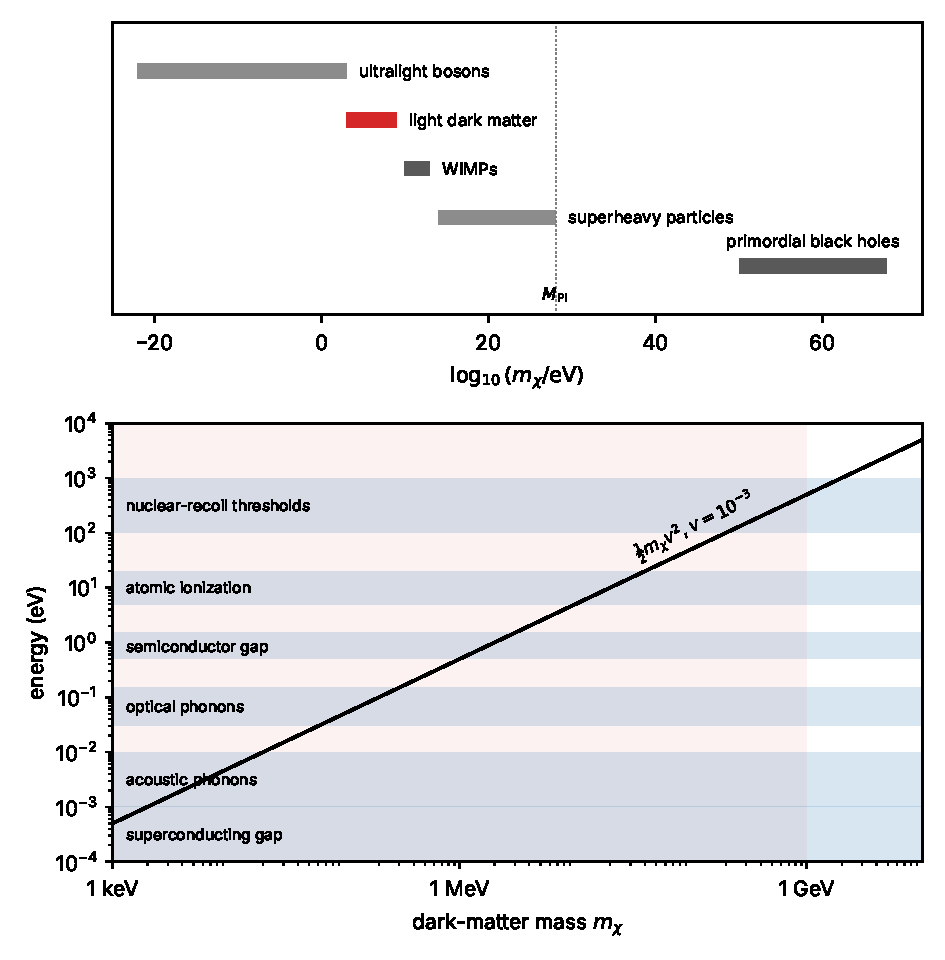
\includegraphics[width=\linewidth]{figures/ch01/fig1_1.pdf}
  \caption{Top: masses of dark-matter candidates, from ultralight bosonic fields to primordial black holes; the dotted line marks the Planck mass. Ranges follow Ref.~\cite[Sect.~I]{lin2019tasi}. Bottom: the keV--GeV window (shaded red). The solid line is the kinetic energy $\frac12 m_\chi v^2$ of dark matter moving at $v = 10^{-3}$. The blue bands are the energy scales of excitations in solids and the thresholds of nuclear-recoil detectors~\cite{kahn2022searches}.}
  \label{fig:1-massrange}
\end{figure}

Within this range, the window between a keV and a GeV has been tested least. Dark matter bound to the Galaxy moves at $v \approx 10^{-3}$, so its kinetic energy $\frac12 \mchi v^2$ is \SI{0.5}{keV} for \SI{1}{GeV}, \SI{0.5}{eV} for \SI{1}{MeV} and \SI{0.5}{meV} for \SI{1}{keV}. A \SI{1}{GeV} particle can deposit at most about \SI{0.1}{keV} in a xenon nucleus (\cref{sec:1.3}). A deposit of \SI{0.1}{keV} is below the thresholds of ton-scale xenon detectors, which read the scintillation and ionization of the recoiling nucleus: Ref.~\cite[Sect.~I]{kahn2022searches} places these thresholds at the few-hundred-eV scale, and the thresholds of analyses that require both signals lie nearer a keV. Solids, however, have excitations across the range of these kinetic energies: typical electronic band gaps of an eV and optical phonons of tens of meV~\cite[Table~I]{kahn2022searches}, and acoustic phonons and superconducting gaps at the meV scale and below (\cref{sec:1.3,sec:1.5}). Particles in this window, between a keV and a GeV, are what the field calls \emph{light dark matter}, or sub-GeV dark matter.

\section{The local halo}\label{sec:1.2}

Every rate in this book is an average over the dark matter that passes through the detector. That average is fixed by the local mass density, which sets how many particles there are, and by the velocity distribution in the laboratory, which sets how fast they move and from which direction they come.

\subsection{Density and velocity distribution}

Measurements of the local dark-matter density, from the motion of stars near the Sun and from the rotation curve of the Galaxy, give values between 0.2 and \SI{0.6}{GeV.cm^{-3}}~\cite[Sect.~3.1.1]{baxter2021recommended}. Mass models with different halo shapes and data sets disagree by more than their statistical errors~\cite[Sect.~3.1]{green2012astrophysical}. For this reason direct-detection results are quoted for a fixed reference value; we use the recommended one~\cite[Table~1]{baxter2021recommended},
\begin{equation}
  \rho_\chi = \SI{0.3}{GeV.cm^{-3}} = \SI{2.31e-6}{eV^4},
  \label{eq:1.2-rho}
\end{equation}
where the value in natural units follows from multiplying by $(\hbar c)^3$, with $\hbar c = \SI{1.973e-5}{eV.cm}$ (\cref{app:A.1}). Since the density enters every rate as an overall factor, a different value rescales a limit without changing its shape~\cite[Sect.~3.1.1]{baxter2021recommended}. The number density of particles of mass $m_\chi$ is $\nd_\chi = \rho_\chi/m_\chi$: three particles per cubic centimeter at \SI{100}{MeV}, three thousand at \SI{100}{keV}. For comparison, \SI{0.3}{GeV.cm^{-3}} is the mass of one hydrogen atom in roughly \SI{3}{cm^3}, while a crystal holds about $10^{23}$ atoms in each cubic centimeter.

The velocity distribution is modeled first in the rest frame of the Galaxy, in which the halo as a whole does not rotate. We write $\vect{v}_{\mathrm{gal}}$ for a dark-matter velocity in that frame and use Cartesian galactic axes: the first points from the Sun to the Galactic center, the second along the direction of Galactic rotation, and the third to the north Galactic pole~\cite[Sect.~5]{green2012astrophysical}. The \emph{standard halo model} (SHM) takes the halo to be a singular isothermal sphere, a self-gravitating gas with density $\rho_{\mathrm{halo}}(r) \propto r^{-2}$ at galactocentric radius $r$, which encloses a mass growing linearly with $r$ and so gives the flat rotation curve of \cref{sec:1.1}~\cite[Sect.~2.1]{green2012astrophysical}. Its particles have an isotropic Maxwellian distribution,
\begin{equation}
  f_{\mathrm{gal}}(\vect{v}_{\mathrm{gal}}) = \frac{1}{N_{\mathrm{esc}}}\, \ee^{-v_{\mathrm{gal}}^2/v_0^2}\, \Theta(v_{\mathrm{esc}} - v_{\mathrm{gal}}),
  \label{eq:1.2-fgal}
\end{equation}
normalized to $\int \dd^3 v_{\mathrm{gal}}\, f_{\mathrm{gal}} = 1$, with $v_{\mathrm{gal}} = |\vect{v}_{\mathrm{gal}}|$ and $\Theta(x)$ the Heaviside step function~\cite[Eq.~(10)]{baxter2021recommended}. It is specified by the speed parameter $v_0$ and the escape speed $v_{\mathrm{esc}}$, which together fix the normalization $N_{\mathrm{esc}}$.

The speed parameter $v_0$ is the local circular speed. Each Cartesian component of $\vect{v}_{\mathrm{gal}}$ in \cref{eq:1.2-fgal} has variance $v_0^2/2$, and for $\rho_{\mathrm{halo}} \propto r^{-2}$ the Jeans equation, which balances the gradient of the velocity pressure $\rho_{\mathrm{halo}} v_0^2/2$ against gravity, gives $v_0 = v_{\mathrm{c}}$~\cite[Eq.~(11)]{green2012astrophysical}. We take the speed of the local standard of rest, the circular orbit at the Sun's radius, $v_0 = \SI{238}{km.s^{-1}}$ (\cref{tab:1-shm}).

The escape speed $v_{\mathrm{esc}}$ truncates the distribution. A particle faster than the local escape speed is not bound to the Galaxy and is assumed absent. Since the isothermal sphere itself has an infinite escape speed, the cut is imposed by hand, and the sharp step is an idealization~\cite[Sect.~2.1]{green2012astrophysical}. The value $v_{\mathrm{esc}} = \SI{544}{km.s^{-1}}$ comes from the fastest stars in the Radial Velocity Experiment (RAVE) survey; later surveys give medians from 485 to \SI{580}{km.s^{-1}}~\cite[Sect.~3.1.2 and Table~2]{baxter2021recommended}.

The normalization $N_{\mathrm{esc}}$ follows in spherical coordinates~\cite[Eq.~(15)]{griffin2018directional}. Since the integrand depends only on $v_{\mathrm{gal}}$, the angles contribute $4\pi$, and
\begin{equation}
  N_{\mathrm{esc}} = 4\pi \int_0^{v_{\mathrm{esc}}} \dd y\, y^2 \ee^{-y^2/v_0^2}
  = \pi^{3/2} v_0^3 \left[\operatorname{erf}\!\left(\frac{v_{\mathrm{esc}}}{v_0}\right) - \frac{2}{\sqrt{\pi}}\,\frac{v_{\mathrm{esc}}}{v_0}\, \ee^{-v_{\mathrm{esc}}^2/v_0^2}\right],
  \label{eq:1.2-nesc}
\end{equation}
with the error function $\operatorname{erf}(x) = (2/\sqrt{\pi})\int_0^x \ee^{-y^2}\dd y$ (\cref{app:C.8}). The second equality integrates $y^2 \ee^{-y^2/v_0^2}$ once by parts; \cref{app:D.1} writes the step out. Without the cut, $N_{\mathrm{esc}}$ would be the Gaussian integral $\pi^{3/2}v_0^3$; the bracket is the fraction of that Gaussian below $v_{\mathrm{esc}}$.

The Sun moves through this distribution. Its velocity in the galactic frame is the circular velocity of the local standard of rest plus the Sun's peculiar motion relative to it~\cite[Table~1 and Eq.~(14)]{baxter2021recommended},
\begin{equation}
  \vect{v}_{\odot} = (0, 238, 0) + (11.1, 12.2, 7.3)\ \si{km.s^{-1}} = (11.1, 250.2, 7.3)\ \si{km.s^{-1}},
  \label{eq:1.2-vsun}
\end{equation}
in the galactic axes above. The magnitude is $|\vect{v}_{\odot}| = (11.1^2 + 250.2^2 + 7.3^2)^{1/2}\,\si{km.s^{-1}} = \SI{250.55}{km.s^{-1}}$, which we round to the reference value $\SI{250.5}{km.s^{-1}}$. \Cref{tab:1-shm} collects the parameters.

\begin{table}[t]
  \centering
  \caption{Standard-halo-model parameters adopted in this book, with their sources. Vectors are given in galactic axes (toward the Galactic center, along Galactic rotation, toward the north Galactic pole). The last two rows follow from the others. The reference Earth speed is the adopted magnitude of the solar velocity $(0, 238, 0) + (11.1, 12.2, 7.3)$\,\si{km.s^{-1}}. The largest laboratory speed adds it to the escape speed.}
  \label{tab:1-shm}
  \begin{tabular}{@{}llll@{}}
    \toprule
    Symbol & Quantity & Value & Source \\
    \midrule
    $\rho_\chi$ & local dark-matter density & \SI{0.3}{GeV.cm^{-3}} & \cite[Table~1]{baxter2021recommended} \\
    $v_0$ & circular speed at the Sun's radius & \SI{238}{km.s^{-1}} & \cite[Table~1]{baxter2021recommended} \\
    $v_{\mathrm{esc}}$ & Galactic escape speed & \SI{544}{km.s^{-1}} & \cite[Table~1]{baxter2021recommended} \\
    -- & solar peculiar velocity & $(11.1, 12.2, 7.3)$\,\si{km.s^{-1}} & \cite[Table~1]{baxter2021recommended} \\
    -- & mean orbital speed of the Earth & \SI{29.8}{km.s^{-1}} & \cite[Eq.~(13)]{baxter2021recommended} \\
    $\vect{v}_\oplus(t)$ & Earth velocity relative to the Sun & \cref{eq:1.2-vorb} & \cite[Eq.~(11)]{baxter2021recommended} \\
    $v_{\mathrm{E}}^{\mathrm{ref}}$ & reference Earth speed (adopted $|\vect{v}_\odot|$) & \SI{250.5}{km.s^{-1}} & \cref{eq:1.2-vsun} \\
    $v_{\mathrm{max}}$ & largest laboratory speed $v_{\mathrm{esc}} + v_{\mathrm{E}}^{\mathrm{ref}}$ & \SI{794.5}{km.s^{-1}} & \cref{eq:1.2-vmax} \\
    \bottomrule
  \end{tabular}
\end{table}

\subsection{The laboratory frame}

A detector shares the motion of the Earth. Its velocity in the galactic frame is
\begin{equation}
  \vect{v}_{\mathrm{E}}(t) = \vect{v}_{\odot} + \vect{v}_{\oplus}(t),
  \label{eq:1.2-vE}
\end{equation}
where $\vect{v}_{\oplus}(t)$ is the Earth's orbital velocity relative to the Sun. Since galactic speeds are below $10^{-2}$ in natural units, the change of frame is Galilean, with relativistic corrections of relative size $v^2 \approx 10^{-6}$. A particle with laboratory velocity $\vect{v}$ has galactic velocity
\begin{equation}
  \vect{v}_{\mathrm{gal}} = \vect{v} + \vect{v}_{\mathrm{E}}(t).
  \label{eq:1.2-galilean}
\end{equation}
The shift has unit Jacobian, $\dd^3 v_{\mathrm{gal}} = \dd^3 v$, and a velocity cell holds the same number of particles in both frames. The laboratory distribution is the galactic one of \cref{eq:1.2-fgal}~\cite[Eq.~(10)]{baxter2021recommended} evaluated at the boosted velocity, $f_\chi(\vect{v}) = f_{\mathrm{gal}}(\vect{v} + \vect{v}_{\mathrm{E}}(t))$:
\begin{equation}
  f_\chi(\vect{v}, t) = \frac{1}{N_{\mathrm{esc}}}\, \ee^{-|\vect{v} + \vect{v}_{\mathrm{E}}(t)|^2/v_0^2}\, \Theta\bigl(v_{\mathrm{esc}} - |\vect{v} + \vect{v}_{\mathrm{E}}(t)|\bigr).
  \label{eq:1.2-flab}
\end{equation}
We write $f_\chi(\vect{v})$ when the time is not needed, and $v = |\vect{v}|$ for the laboratory speed. The normalization is unchanged, $\int\dd^3 v\, f_\chi = 1$, and we write angle brackets for an average over the distribution, $\langle\cdots\rangle = \int \dd^3 v\, f_\chi(\vect{v})\,(\cdots)$. In the laboratory the distribution is no longer centered on zero: the most probable velocity is $-\vect{v}_{\mathrm{E}}$. Dark matter arrives as a wind from the direction in which the Earth moves. Because $f_{\mathrm{gal}}$ is even in $\vect{v}_{\mathrm{gal}}$, its mean velocity vanishes, and by \cref{eq:1.2-galilean} the mean laboratory velocity is exactly $\langle\vect{v}\rangle = -\vect{v}_{\mathrm{E}}(t)$, cut or no cut.

The spread about this mean is the galactic one: $\langle v_{\mathrm{gal}}^2\rangle^{1/2} = (3/2)^{1/2} v_0 = \SI{291}{km.s^{-1}}$ for the Gaussian and \SI{284}{km.s^{-1}} with the cut. The spread is larger than the drift: the wind is broad. A numerical integration of \cref{eq:1.2-flab} at $v_{\mathrm{E}} = v_{\mathrm{E}}^{\mathrm{ref}}$ shows that \SI{94}{\percent} of the particles move with a positive component along $-\vect{v}_{\mathrm{E}}$, and \SI{59}{\percent} within $45^\circ$ of it; the mean cosine of the angle to $-\vect{v}_{\mathrm{E}}$ is 0.66.

The fastest particle in the laboratory is one that moves at $v_{\mathrm{esc}}$ in the galactic frame, opposite to $\vect{v}_{\mathrm{E}}$; its laboratory speed is $v_{\mathrm{esc}} + |\vect{v}_{\mathrm{E}}(t)|$. We quote thresholds and kinematic edges at a fixed reference speed, the rounded solar speed $v_{\mathrm{E}}^{\mathrm{ref}} = \SI{250.5}{km.s^{-1}}$ (\cref{eq:1.2-vsun}; \cref{app:A.8}). The \emph{maximum speed} is then
\begin{equation}
  v_{\mathrm{max}} = v_{\mathrm{esc}} + v_{\mathrm{E}}^{\mathrm{ref}} = \SI{794.5}{km.s^{-1}} = 2.650\times10^{-3}.
  \label{eq:1.2-vmax}
\end{equation}
Over a year $v_{\mathrm{esc}} + |\vect{v}_{\mathrm{E}}(t)|$ ranges from 781 to \SI{810}{km.s^{-1}} (see the annual modulation below). With the reference value, thresholds stay time-independent, while integrals over $f_\chi$ use the full $\vect{v}_{\mathrm{E}}(t)$, averaged over the exposure.

Many rates depend only on the speed. The \emph{speed distribution} $F_\chi(v)$, normalized to $\int_0^\infty \dd v\, F_\chi = 1$, is $v^2$ times the integral of $f_\chi$ over directions. Take the polar axis along $\vect{v}_{\mathrm{E}}$, write $\vartheta$ for the angle between $\vect{v}$ and $\vect{v}_{\mathrm{E}}$, and $v_{\mathrm{E}} = |\vect{v}_{\mathrm{E}}|$. Then $|\vect{v} + \vect{v}_{\mathrm{E}}|^2 = v^2 + v_{\mathrm{E}}^2 + 2 v v_{\mathrm{E}} \cos\vartheta$, and the azimuth contributes $2\pi$:
\begin{equation*}
  F_\chi(v) = \frac{2\pi v^2}{N_{\mathrm{esc}}}\, \ee^{-(v^2 + v_{\mathrm{E}}^2)/v_0^2} \int_{-1}^{\cos\vartheta_{\mathrm{cut}}} \dd (\cos\vartheta)\, \ee^{-2 v v_{\mathrm{E}} \cos\vartheta/v_0^2}.
\end{equation*}
The upper limit $\cos\vartheta_{\mathrm{cut}}$ is where $|\vect{v} + \vect{v}_{\mathrm{E}}| = v_{\mathrm{esc}}$, or 1 if that never happens. For $v < v_{\mathrm{esc}} - v_{\mathrm{E}}$ no direction reaches the cut and $\cos\vartheta_{\mathrm{cut}} = 1$. For $v_{\mathrm{esc}} - v_{\mathrm{E}} < v < v_{\mathrm{esc}} + v_{\mathrm{E}}$ the cut removes the directions close to $\vect{v}_{\mathrm{E}}$, and at $\cos\vartheta_{\mathrm{cut}}$ the exponent equals $-v_{\mathrm{esc}}^2/v_0^2$. Doing the elementary integral, we find
\begin{equation}
  F_\chi(v) = \frac{\pi v_0^2\, v}{v_{\mathrm{E}} N_{\mathrm{esc}}} \times
  \begin{cases}
    \ee^{-(v - v_{\mathrm{E}})^2/v_0^2} - \ee^{-(v + v_{\mathrm{E}})^2/v_0^2}, & v < v_{\mathrm{esc}} - v_{\mathrm{E}},\\[2pt]
    \ee^{-(v - v_{\mathrm{E}})^2/v_0^2} - \ee^{-v_{\mathrm{esc}}^2/v_0^2}, & v_{\mathrm{esc}} - v_{\mathrm{E}} < v < v_{\mathrm{esc}} + v_{\mathrm{E}}
  \end{cases},
  \label{eq:1.2-Fspeed}
\end{equation}
and $F_\chi = 0$ above $v_{\mathrm{esc}} + v_{\mathrm{E}}$. The two branches join continuously at $v = v_{\mathrm{esc}} - v_{\mathrm{E}}$, and the second vanishes at $v_{\mathrm{esc}} + v_{\mathrm{E}}$. \Cref{eq:1.2-Fspeed} assumes $v_{\mathrm{E}} < v_{\mathrm{esc}}$, which holds by a factor of two. \Cref{fig:1-speed} shows $F_\chi$ on the days of largest and smallest Earth speed. In the galactic frame the speed distribution $4\pi v_{\mathrm{gal}}^2 f_{\mathrm{gal}}$ peaks at $v_0$; in the laboratory the drift moves the peak to \SI{335}{km.s^{-1}} (at $v_{\mathrm{E}} = v_{\mathrm{E}}^{\mathrm{ref}}$) and stretches the tail to $v_{\mathrm{esc}} + v_{\mathrm{E}}$.

\begin{figure}[tbp]
  \centering
  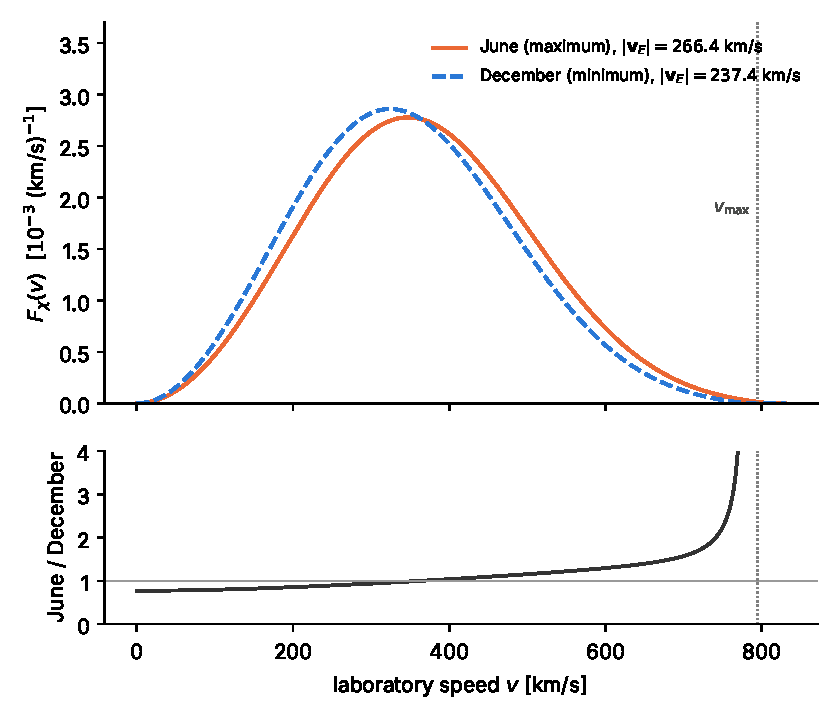
\includegraphics[width=0.85\linewidth]{figures/ch01/fig1_3.pdf}
  \caption{Top: laboratory-frame speed distribution $F_\chi(v)$ of the standard halo model with $v_0 = \SI{238}{km.s^{-1}}$ and $v_{\mathrm{esc}} = \SI{544}{km.s^{-1}}$, in June (solid, Earth speed at its annual maximum \SI{266.4}{km.s^{-1}}) and December (dashed, \SI{237.4}{km.s^{-1}}), the days of largest and smallest Earth speed for the Earth velocity of \cref{eq:1.2-vorb}~\cite[Eq.~(11)]{baxter2021recommended}. Bottom: ratio of the June to the December distribution. The dotted line marks $v_{\mathrm{max}} = \SI{794.5}{km.s^{-1}}$; in June the distribution extends to \SI{810}{km.s^{-1}}, in December to \SI{781}{km.s^{-1}}.}
  \label{fig:1-speed}
\end{figure}

The tail of $F_\chi$ matters for light dark matter, which must often use the fastest particles to deposit enough energy (\cref{sec:1.3}). We integrate \cref{eq:1.2-Fspeed} numerically at $v_{\mathrm{E}} = v_{\mathrm{E}}^{\mathrm{ref}}$. The fraction of particles faster than 400, 500, 600 and \SI{700}{km.s^{-1}} is \SI{36}{\percent}, \SI{15}{\percent}, \SI{4.2}{\percent} and \SI{0.58}{\percent}; above \SI{750}{km.s^{-1}} it is \SI{0.10}{\percent}. A threshold that needs $v \gtrsim \SI{700}{km.s^{-1}}$ sees a rate suppressed by more than two orders of magnitude, and one that depends on $v_{\mathrm{esc}}$ and on the exact shape of the cut, the most uncertain parts of the model.

Scattering rates contain the speed through $1/v$: the energy-conservation delta function of a collision, integrated over the direction of $\vect{v}$, leaves a factor $1/v$ (\cref{sec:1.3}). In the SHM this average has a closed form.

\begin{workedexample}{Normalization and mean inverse speed}\label{we:1-nesc}
With $v_{\mathrm{esc}}/v_0 = 544/238 = 2.286$, the error function is $\operatorname{erf}(2.286) = 0.99877$ and the second term in the bracket of \cref{eq:1.2-nesc} is $(2/\sqrt{\pi})(2.286)\,\ee^{-5.224} = 2.579 \times 0.005383 = 0.01388$. The bracket is $0.98489$: the cut removes \SI{1.5}{\percent} of the Gaussian. With $\pi^{3/2} v_0^3 = 5.5683 \times (238)^3\,\si{(km/s)^3} = \SI{7.507e7}{(km/s)^3}$,
\begin{equation*}
  N_{\mathrm{esc}} = 0.98489 \times \SI{7.507e7}{(km/s)^3} = \SI{7.393e7}{(km/s)^3}.
\end{equation*}
The mean inverse speed is $\langle 1/v\rangle = \int_0^\infty \dd v\, F_\chi(v)/v$. Dividing \cref{eq:1.2-Fspeed} by $v$ leaves Gaussians in $v \mp v_{\mathrm{E}}$ and a constant. Substituting $y = v - v_{\mathrm{E}}$ in the first exponential and $y = v + v_{\mathrm{E}}$ in the second, the two cancel on $v_{\mathrm{E}} < y < v_{\mathrm{esc}}$ and leave $\int_{-v_{\mathrm{E}}}^{v_{\mathrm{E}}} \ee^{-y^2/v_0^2}\dd y = \sqrt{\pi}\, v_0 \operatorname{erf}(v_{\mathrm{E}}/v_0)$; the constant term, integrated over an interval of length $2v_{\mathrm{E}}$, contributes $-2 v_{\mathrm{E}} \ee^{-v_{\mathrm{esc}}^2/v_0^2}$ (\cref{app:D.1}). Hence
\begin{equation}
  \left\langle \frac{1}{v} \right\rangle = \frac{\pi v_0^2}{v_{\mathrm{E}} N_{\mathrm{esc}}} \left[\sqrt{\pi}\, v_0 \operatorname{erf}\!\left(\frac{v_{\mathrm{E}}}{v_0}\right) - 2 v_{\mathrm{E}}\, \ee^{-v_{\mathrm{esc}}^2/v_0^2}\right].
  \label{eq:1.2-inv}
\end{equation}
At $v_{\mathrm{E}} = v_{\mathrm{E}}^{\mathrm{ref}} = \SI{250.5}{km.s^{-1}}$, $v_{\mathrm{E}}/v_0 = 1.0525$ and $\operatorname{erf}(1.0525) = 0.86338$. The bracket is $\sqrt{\pi} \times 238 \times 0.86338 - 2 \times 250.5 \times 0.005383 = 364.21 - 2.70 = \SI{361.51}{km.s^{-1}}$, and the prefactor is $\pi (238)^2/(250.5 \times \SI{7.393e7}{}) = \SI{9.608e-6}{(km/s)^{-2}}$. The result is
\begin{equation*}
  \left\langle \frac{1}{v} \right\rangle = \SI{3.474e-3}{(km/s)^{-1}} = \frac{1}{\SI{287.9}{km.s^{-1}}}, \quad\text{or } 1041 \text{ in natural units}.
\end{equation*} Without the cut, \cref{eq:1.2-inv} reduces to $\operatorname{erf}(v_{\mathrm{E}}/v_0)/v_{\mathrm{E}} = 1/(\SI{290.1}{km.s^{-1}})$; the cut removes fast particles and raises $\langle 1/v\rangle$ by \SI{0.8}{\percent}. In June and December the same formula yields $1/(\SI{298.3}{km.s^{-1}})$ and $1/(\SI{279.8}{km.s^{-1}})$, a \SI{6}{\percent} swing.
\end{workedexample}

The mean inverse speed is the value at zero of the function $\eta(\vmin) = \langle \Theta(v - \vmin)/v\rangle$ that \cref{sec:1.3} introduces, with $\vmin$ the minimum velocity of \cref{eq:1.3-vmin}; \cref{app:D.1} gives $\eta$ for every $\vmin$.

\subsection{Annual modulation}

The Earth's orbital velocity, in the galactic axes of \cref{eq:1.2-vsun}, is~\cite[Eq.~(11)]{baxter2021recommended}
\begin{equation}
  \vect{v}_{\oplus}(t) = \SI{29.8}{km.s^{-1}} \left[\begin{pmatrix} 0.9941\\ 0.1088\\ 0.0042 \end{pmatrix} \cos \omega_{\mathrm{yr}} t + \begin{pmatrix} -0.0504\\ 0.4946\\ -0.8677 \end{pmatrix} \sin \omega_{\mathrm{yr}} t \right],
  \label{eq:1.2-vorb}
\end{equation}
with $\omega_{\mathrm{yr}} = \SI{0.0172}{d^{-1}}$ the orbital angular frequency and $t$ counted in days from 22 March. The two column vectors are orthogonal unit vectors, to $10^{-4}$, that span the plane of the orbit, and \SI{29.8}{km.s^{-1}} is the mean orbital speed~\cite[Eq.~(13)]{baxter2021recommended}. We treat the orbit as a circle; its eccentricity moves the date of the largest Earth speed by 1.2 days and the modulation amplitude by \SI{0.4}{\percent}~\cite[Table~I]{mccabe2014earth}, both too small to matter here.

Since the orbital speed is small next to the solar speed, $29.8/250.5 = 0.12$, we can expand the Earth's speed to first order in it:
\begin{equation*}
  |\vect{v}_{\mathrm{E}}(t)| = \bigl(|\vect{v}_\odot|^2 + 2\vect{v}_\odot\cdot\vect{v}_\oplus + |\vect{v}_\oplus|^2\bigr)^{1/2} \approx v_{\mathrm{E}}^{\mathrm{ref}} + \hat{\vect{v}}_\odot \cdot \vect{v}_\oplus(t),
\end{equation*}
with $\hat{\vect{v}}_\odot = \vect{v}_\odot/|\vect{v}_\odot| = (0.0443, 0.9986, 0.0291)$ from \cref{eq:1.2-vsun}. Projected onto $\hat{\vect{v}}_\odot$, the two vectors of \cref{eq:1.2-vorb} have components $0.1528$ and $0.4664$, and
\begin{equation}
  |\vect{v}_{\mathrm{E}}(t)| \approx v_{\mathrm{E}}^{\mathrm{ref}} + \SI{14.6}{km.s^{-1}} \cos\bigl[\omega_{\mathrm{yr}}(t - t_{\mathrm{peak}})\bigr],
  \label{eq:1.2-annual}
\end{equation}
with amplitude $29.8 \times (0.1528^2 + 0.4664^2)^{1/2} = 29.8 \times 0.4908 = \SI{14.6}{km.s^{-1}}$ and phase $\omega_{\mathrm{yr}} t_{\mathrm{peak}} = \arctan(0.4664/0.1528) = 71.9^\circ = \SI{1.254}{rad}$, which is $t_{\mathrm{peak}} = 72.9$ days after 22 March, that is, 2 June. Only half of the orbital speed modulates the Earth's speed because the Sun's velocity makes an angle of $\arccos 0.4908 = 60.6^\circ$ with the plane of the orbit. The second-order term, $(|\vect{v}_\oplus|^2 - (\hat{\vect{v}}_\odot\cdot\vect{v}_\oplus)^2)/(2v_{\mathrm{E}}^{\mathrm{ref}})$, adds \SI{1.3}{km.s^{-1}} at both extremes and \SI{1.6}{km.s^{-1}} on average over the year. The exact speed from \cref{eq:1.2-vE,eq:1.2-vorb} is largest on 2 June, \SI{266.4}{km.s^{-1}}, smallest on 2 December, \SI{237.4}{km.s^{-1}}, and averages \SI{252.1}{km.s^{-1}} over the year.

The rate follows the change of $F_\chi$ with the season, and its sign depends on which speeds the process can use. In June the distribution is shifted to higher speeds: it holds more particles above \SI{364}{km.s^{-1}}, where the curves of \cref{fig:1-speed} cross, and fewer below. A rate that needs fast particles, such as one near a kinematic threshold, peaks in June. A rate that weights all speeds by $1/v$ peaks in December, since $\langle 1/v \rangle$ is \SI{6}{\percent} larger then (\cref{we:1-nesc}). For the integral $\eta(\vmin)$ of \cref{sec:1.3}, built from \cref{app:D.1}, the phase reverses at $\vmin = \SI{211}{km.s^{-1}}$; above, the modulation grows from a few percent to $+\SI{21}{\percent}$ and $\SI{-16}{\percent}$ about the reference value at $\vmin = \SI{600}{km.s^{-1}}$, and to $+\SI{42}{\percent}$ and $\SI{-28}{\percent}$ at \SI{700}{km.s^{-1}}. Averaged over the year, $\langle 1/v\rangle$ lies \SI{0.3}{\percent} below its value at $v_{\mathrm{E}}^{\mathrm{ref}}$ and agrees to $10^{-4}$ with its value at the annual-mean speed. In the tail the difference grows: at $\vmin = 600$ and \SI{700}{km.s^{-1}} the yearly average of $\eta$ exceeds its value at $v_{\mathrm{E}}^{\mathrm{ref}}$ by \SI{2.6}{\percent} and \SI{5.6}{\percent}, because $\eta$ there is a convex function of $v_{\mathrm{E}}$.

The size of the modulation follows from the closed forms by differentiation. For a rate that depends on time only through $v_{\mathrm{E}}$, \cref{eq:1.2-annual} makes the relative modulation about the yearly mean
\begin{equation*}
  (\SI{14.6}{km.s^{-1}})\,\frac{\partial \ln(\text{rate})}{\partial v_{\mathrm{E}}}\, \cos\bigl[\omega_{\mathrm{yr}}(t - t_{\mathrm{peak}})\bigr],
\end{equation*}
with the derivative taken at $v_{\mathrm{E}}^{\mathrm{ref}}$. For a rate proportional to $\langle 1/v\rangle$, write \cref{eq:1.2-inv} as $\pi v_0^2 \mathcal{I}(v_{\mathrm{E}})/(v_{\mathrm{E}} N_{\mathrm{esc}})$ with $\mathcal{I}(v_{\mathrm{E}})$ the bracket. Since $\dd \operatorname{erf}(x)/\dd x = (2/\sqrt{\pi})\ee^{-x^2}$, $\dd \mathcal{I}/\dd v_{\mathrm{E}} = 2\ee^{-v_{\mathrm{E}}^2/v_0^2} - 2\ee^{-v_{\mathrm{esc}}^2/v_0^2} = 0.6498$, and
\begin{equation*}
  \frac{\partial \ln\langle 1/v\rangle}{\partial v_{\mathrm{E}}} = -\frac{1}{v_{\mathrm{E}}} + \frac{1}{\mathcal{I}}\frac{\dd \mathcal{I}}{\dd v_{\mathrm{E}}} = -\frac{1}{250.5} + \frac{0.6498}{361.51} = \SI{-2.195e-3}{(km/s)^{-1}}.
\end{equation*}
The amplitude is $14.6 \times (-2.195\times10^{-3}) = \SI{-3.2}{\percent}$: the mean inverse speed is largest in December (\cref{we:1-nesc}).

Annual modulation is a signature because each of its features is fixed by the halo and the orbit, not by the detector. The period is one year, the phase is set by the June maximum and December minimum, the phase flips at a definite $\vmin$, and the amplitude grows toward the kinematic edge. A background would have to reproduce all four. The amplitude is also more sensitive to the shape of the speed distribution than the time-averaged rate is, and an observed modulation would test the halo model itself~\cite[Sect.~6.2]{green2012astrophysical}.

\subsection{Daily modulation}

The Earth also rotates, and a crystal fixed in the laboratory turns with it relative to $\vect{v}_{\mathrm{E}}$. The rotation speed, $2\pi \times \SI{6378}{km}/\SI{86164}{s} = \SI{0.47}{km.s^{-1}}$ at the equator and less by the cosine of the latitude elsewhere, is \SI{3}{\percent} of the annual amplitude of \cref{eq:1.2-annual} and leaves the speed distribution practically unchanged. What changes, however, is the direction from which the wind arrives in crystal axes.

The rotation is simplest in equatorial coordinates. Their Cartesian axes are fixed relative to the distant stars: the third points along the Earth's rotation axis to the north celestial pole, the first to the vernal equinox in the celestial equator, and the second completes a right-handed set. A direction on the sky is given by its \emph{declination}, the angle above the celestial equator, and its \emph{right ascension}, the angle measured eastward in the equatorial plane from the vernal equinox. Right ascension is often quoted in hours ($\SI{24}{h} = 360^\circ$). In equatorial Cartesian axes a direction has the polar angle $90^\circ$ minus its declination and the azimuth equal to its right ascension. A laboratory turns about the third axis once per sidereal day, the rotation period relative to the stars. Its \emph{meridian} is the half-plane bounded by the rotation axis that contains the local vertical, its \emph{local sidereal time} is the right ascension of that meridian, and the \emph{hour angle} of a direction is the local sidereal time minus the direction's right ascension.

The rotation from equatorial to galactic Cartesian axes is fixed by three angles: the equatorial coordinates of the north Galactic pole, right ascension $192.85948^\circ$ and declination $27.12825^\circ$, and the galactic longitude of the north celestial pole, $122.932^\circ$~\cite[App.~B, Eq.~(B3)]{mccabe2014earth}. Built from these angles, it takes a unit vector with equatorial components $(x_{\mathrm{eq}}, y_{\mathrm{eq}}, z_{\mathrm{eq}})$ to its galactic components,
\begin{equation}
  \begin{pmatrix} x_{\mathrm{gal}}\\ y_{\mathrm{gal}}\\ z_{\mathrm{gal}} \end{pmatrix}
  = \begin{pmatrix} -0.0549 & -0.8734 & -0.4838\\ 0.4941 & -0.4448 & 0.7470\\ -0.8677 & -0.1981 & 0.4560 \end{pmatrix}
  \begin{pmatrix} x_{\mathrm{eq}}\\ y_{\mathrm{eq}}\\ z_{\mathrm{eq}} \end{pmatrix}.
  \label{eq:1.2-rotation}
\end{equation}
The rows are the galactic axes in equatorial components; the first, the direction of the Galactic center, has right ascension $266.4^\circ$ and declination $-28.9^\circ$. The third column is the north celestial pole in galactic axes. Its scalar product with $\hat{\vect{v}}_\odot$ is $0.7378$, which means the solar velocity makes the angle
\begin{equation}
  \theta_{\mathrm{E}} = \arccos 0.7378 = 42.5^\circ,
  \label{eq:1.2-thetaE}
\end{equation}
with the rotation axis. The transpose of \cref{eq:1.2-rotation}, which is its inverse, takes $\hat{\vect{v}}_\odot$ to the equatorial components $(0.4657, -0.4887, 0.7378)$, that is, right ascension $\arctan(-0.4887/0.4657) + 360^\circ = 313.6^\circ =$ \SI{20.9}{h} and declination $47.5^\circ = 90^\circ - \theta_{\mathrm{E}}$, in the constellation Cygnus. The orbital motion moves this direction during the year, to declination $42.8^\circ$ in June and $52.6^\circ$ in December, so the angle to the rotation axis varies between $47.2^\circ$ and $37.4^\circ$. We use $\hat{\vect{v}}_\odot$ below; a prediction at the level of a few degrees computes the direction of $\vect{v}_{\mathrm{E}}(t)$ from \cref{eq:1.2-vE,eq:1.2-vorb} on each day, which combines the annual and daily modulations.

Let $\hat{\vect{n}}$ be an axis fixed in the laboratory, for example a crystal axis, at polar angle $\theta_{\hat{n}}$ from the north celestial pole. As the Earth turns, $\hat{\vect{n}}$ keeps its polar angle and its right ascension advances at the sidereal rate $\omega_{\mathrm{sid}} = 2\pi/(\SI{23}{h}\,\SI{56}{min}\,\SI{4}{s})$. In equatorial Cartesian axes the two unit vectors are $\hat{\vect{v}}_\odot = (\sin\theta_{\mathrm{E}}\cos\alpha_{\mathrm{E}}, \sin\theta_{\mathrm{E}}\sin\alpha_{\mathrm{E}}, \cos\theta_{\mathrm{E}})$, with $\alpha_{\mathrm{E}}$ its right ascension, and $\hat{\vect{n}}(t) = (\sin\theta_{\hat{n}}\cos\alpha_{\hat{n}}(t), \sin\theta_{\hat{n}}\sin\alpha_{\hat{n}}(t), \cos\theta_{\hat{n}})$, with $\alpha_{\hat{n}}(t) = \alpha_{\mathrm{E}} + \omega_{\mathrm{sid}}(t - t_{\mathrm{E}})$ and $t_{\mathrm{E}}$ the time at which both lie in one meridian plane. Their scalar product fixes the angle $\theta_{\mathrm{lab}}(t)$ between $\vect{v}_{\mathrm{E}}$ and the laboratory axis,
\begin{equation}
  \cos\theta_{\mathrm{lab}}(t) = \cos\theta_{\mathrm{E}}\cos\theta_{\hat{n}} + \sin\theta_{\mathrm{E}}\sin\theta_{\hat{n}} \cos\bigl[\omega_{\mathrm{sid}}(t - t_{\mathrm{E}})\bigr].
  \label{eq:1.2-angle}
\end{equation}
Over one sidereal day $\theta_{\mathrm{lab}}$ oscillates between $|\theta_{\mathrm{E}} - \theta_{\hat{n}}|$ and $\theta_{\mathrm{E}} + \theta_{\hat{n}}$ (for $\theta_{\mathrm{E}} + \theta_{\hat{n}} \le 180^\circ$). An axis along the rotation axis, $\theta_{\hat{n}} = 0$, keeps the fixed angle $\theta_{\mathrm{E}}$; an axis in the equatorial plane swings between $47.5^\circ$ and $132.5^\circ$. For the local vertical at latitude $\ell_{\mathrm{lat}}$ north, $\theta_{\hat{n}} = 90^\circ - \ell_{\mathrm{lat}}$ and $\alpha_{\hat{n}}$ is the local sidereal time. \Cref{fig:1-daily} plots \cref{eq:1.2-angle} for the vertical at four latitudes. At $45^\circ$N the angle runs from $2.5^\circ$, when Cygnus is nearly overhead and the wind comes from above, to $87.5^\circ$ twelve sidereal hours later.

A crystal is usually mounted with its axes along the local vertical and the local north and east directions. The full direction of $\hat{\vect{v}}_\odot$ in these axes follows from the same construction. The local vertical at latitude $\ell_{\mathrm{lat}}$ is $(\cos\ell_{\mathrm{lat}}\cos\alpha_{\mathrm{z}}, \cos\ell_{\mathrm{lat}}\sin\alpha_{\mathrm{z}}, \sin\ell_{\mathrm{lat}})$ in equatorial axes, with $\alpha_{\mathrm{z}}$ the local sidereal time. The local north is the derivative of this vector with respect to $\ell_{\mathrm{lat}}$, $(-\sin\ell_{\mathrm{lat}}\cos\alpha_{\mathrm{z}}, -\sin\ell_{\mathrm{lat}}\sin\alpha_{\mathrm{z}}, \cos\ell_{\mathrm{lat}})$. The local east is the unit vector $(-\sin\alpha_{\mathrm{z}}, \cos\alpha_{\mathrm{z}}, 0)$ in the direction of increasing $\alpha_{\mathrm{z}}$. With $\delta_{\mathrm{E}} = 90^\circ - \theta_{\mathrm{E}}$ the declination of $\hat{\vect{v}}_\odot$ and $h_{\mathrm{E}} = \alpha_{\mathrm{z}} - \alpha_{\mathrm{E}}$ its hour angle, the scalar products of these three vectors with $\hat{\vect{v}}_\odot$ are its components
\begin{equation}
  \begin{aligned}
    \hat{v}_{\mathrm{east}} &= -\cos\delta_{\mathrm{E}}\sin h_{\mathrm{E}},\\
    \hat{v}_{\mathrm{north}} &= \cos\ell_{\mathrm{lat}}\sin\delta_{\mathrm{E}} - \sin\ell_{\mathrm{lat}}\cos\delta_{\mathrm{E}}\cos h_{\mathrm{E}},\\
    \hat{v}_{\mathrm{up}} &= \sin\ell_{\mathrm{lat}}\sin\delta_{\mathrm{E}} + \cos\ell_{\mathrm{lat}}\cos\delta_{\mathrm{E}}\cos h_{\mathrm{E}}
  \end{aligned},
  \label{eq:1.2-local}
\end{equation}
with $h_{\mathrm{E}} = \omega_{\mathrm{sid}}(t - t_{\mathrm{E}})$ advancing at the sidereal rate. The vertical component is \cref{eq:1.2-angle} for $\theta_{\hat{n}} = 90^\circ - \ell_{\mathrm{lat}}$. At $45^\circ$N and $h_{\mathrm{E}} = 0$ the (east, north, up) components are $(0, 0.04, 1.00)$, a nearly vertical direction; six sidereal hours later, $h_{\mathrm{E}} = 90^\circ$, they are $(-0.67, 0.52, 0.52)$, toward the northwest at $31^\circ$ above the horizon. The wind arrives from the direction $\hat{\vect{v}}_\odot$; the dark-matter velocities point along $-\hat{\vect{v}}_\odot$.

\begin{figure}[tbp]
  \centering
  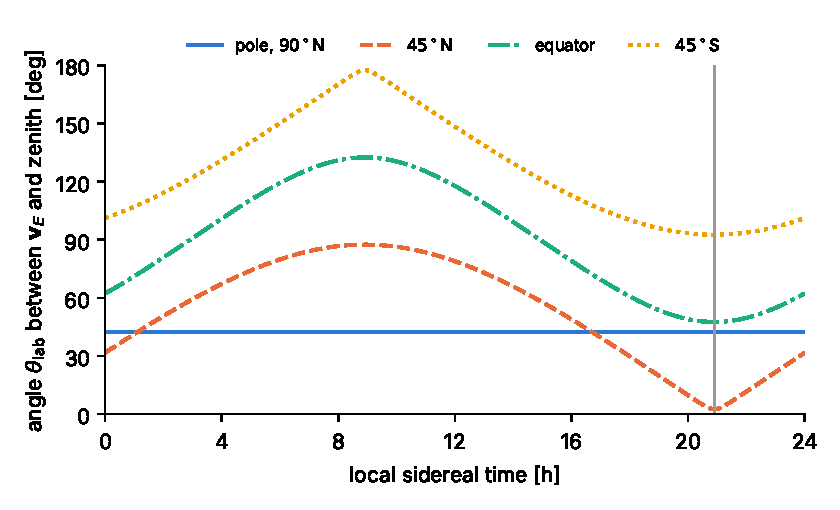
\includegraphics[width=0.85\linewidth]{figures/ch01/fig1_4.pdf}
  \caption{Angle $\theta_{\mathrm{lab}}$ between the Earth's galactic-frame velocity and the local vertical over one sidereal day, as a function of local sidereal time, at latitudes $90^\circ$N, $45^\circ$N, $0^\circ$ and $45^\circ$S. The velocity direction is that of the solar velocity, right ascension \SI{20.9}{h} and declination $47.5^\circ$ (vertical line: its transit), from Ref.~\cite[Table~1]{baxter2021recommended} and the coordinate rotation of Ref.~\cite[Eq.~(B3)]{mccabe2014earth}. The dark-matter wind arrives from this direction.}
  \label{fig:1-daily}
\end{figure}

For an isotropic target, such as a liquid or a polycrystal, the rate depends on $\vect{v}_{\mathrm{E}}$ only through its magnitude, and the rotation changes nothing. A single crystal is anisotropic: its response to a momentum transfer depends on the direction of $\vect{q}$ relative to the crystal axes, and slow dark matter transfers momentum preferentially along the wind. As $\theta_{\mathrm{lab}}$ sweeps through its daily range, the wind samples different crystal directions and the rate varies with the sidereal period.

The simplest anisotropy shows how \cref{eq:1.2-angle} enters a rate. Take a uniaxial crystal, one in which a single axis $\hat{\vect{n}}$ (the optic axis) differs from the two directions perpendicular to it, and whose response is unchanged under $\hat{\vect{n}} \to -\hat{\vect{n}}$. Since the halo of \cref{eq:1.2-flab} is symmetric under rotations about $\vect{v}_{\mathrm{E}}$, after the average over velocities the rate can depend on the two directions only through the scalar $\hat{\vect{n}}\cdot\hat{\vect{v}}_{\mathrm{E}} = \cos\theta_{\mathrm{lab}}$, and evenness in $\hat{\vect{n}}$ makes it a function of $\cos^2\theta_{\mathrm{lab}}$. To lowest order in the anisotropy the rate is a constant plus a constant times $\cos^2\theta_{\mathrm{lab}}(t)$; the crystal response fixes both constants. With the optic axis in the equatorial plane, $\theta_{\hat{n}} = 90^\circ$ and \cref{eq:1.2-angle} reduces to $\cos\theta_{\mathrm{lab}} = \sin\theta_{\mathrm{E}}\cos[\omega_{\mathrm{sid}}(t - t_{\mathrm{E}})]$; $\cos^2\theta_{\mathrm{lab}}$ then swings between 0 and $\sin^2\theta_{\mathrm{E}} = 0.456$ twice each sidereal day. With the optic axis along the Earth's axis the rate is constant.

Polar crystals, whose ions carry opposite charges, show sizable daily modulation of phonon rates when the lattice is strongly anisotropic, as in sapphire, while the cubic crystal GaAs shows almost none. The sidereal period is a distinctive signature: the sidereal day is about four minutes shorter than the solar day, and a background that follows the solar day, or does not vary at all, falls out of phase with the signal over many periods~\cite[Sect.~III\,C]{griffin2018directional}.

\subsection{Number flux}

The number flux of dark matter is the number of particles that cross a unit area per unit time. Each particle is counted across an area perpendicular to its own velocity:
\begin{equation}
  \Phi_\chi = \nd_\chi \langle v \rangle = \frac{\rho_\chi}{m_\chi}\langle v\rangle.
  \label{eq:1.2-flux}
\end{equation}
Multiplied by a velocity-independent cross-section, it is the rate per target particle. A target particle at rest presents a fixed cross-section to each incoming particle, and the particles with velocity in $\dd^3 v$ sweep a volume $v$ per unit time per unit of cross-section; they hit it at the rate $\nd_\chi f_\chi(\vect{v})\,\dd^3 v\, v$ times the cross-section. When the cross-section does not depend on $v$, summing over velocities replaces $v$ by $\langle v\rangle$, and the rate is $\Phi_\chi$ times the cross-section. When it does depend on $v$, as in most of this book, the average must be taken with the cross-section inside, and $\Phi_\chi$ serves only as a measure of how much dark matter passes through. A detector face of fixed orientation intercepts a different number, which depends on the angle between the face and the wind; \cref{eq:1.2-flux} avoids that geometric factor. The mean speed follows from \cref{eq:1.2-Fspeed} as $\langle v\rangle = \int_0^\infty \dd v\, v F_\chi(v)$. It is a sum of Gaussian moments, evaluated in \cref{app:D.1}:
\begin{equation}
  \begin{split}
  \langle v\rangle = \frac{\pi v_0^2}{v_{\mathrm{E}} N_{\mathrm{esc}}} \biggl[& v_{\mathrm{E}} v_0^2\, \ee^{-v_{\mathrm{E}}^2/v_0^2} + \sqrt{\pi}\, v_0\left(\frac{v_0^2}{2} + v_{\mathrm{E}}^2\right)\operatorname{erf}\!\left(\frac{v_{\mathrm{E}}}{v_0}\right)\\
  &- 2 v_{\mathrm{E}}\,\ee^{-v_{\mathrm{esc}}^2/v_0^2}\left(v_0^2 + v_{\mathrm{esc}}^2 + \frac{v_{\mathrm{E}}^2}{3}\right)\biggr]
  \end{split}.
  \label{eq:1.2-vmean}
\end{equation}
Without the cut ($v_{\mathrm{esc}} \to \infty$, $N_{\mathrm{esc}} \to \pi^{3/2}v_0^3$) the bracket loses its last term and \cref{eq:1.2-vmean} becomes the mean speed of a shifted Maxwellian, $v_0[\ee^{-x^2}/\sqrt{\pi} + (x + 1/(2x))\operatorname{erf}x]$ with $x = v_{\mathrm{E}}/v_0$.

\begin{workedexample}{Number flux of \SI{100}{MeV} dark matter}\label{we:1-flux}
We take $v_{\mathrm{E}} = v_{\mathrm{E}}^{\mathrm{ref}}$, so $v_{\mathrm{E}}/v_0 = 1.0525$, $\ee^{-1.1078} = 0.33028$ and $\operatorname{erf}(1.0525) = 0.86338$ (\cref{we:1-nesc}). In units of $(\si{km.s^{-1}})^3$ the three terms in the bracket of \cref{eq:1.2-vmean}, in the order written, are
\begin{align*}
  \text{first:}\quad & 250.5 \times 238^2 \times 0.33028 = \num{4.687e6},\\
  \text{second:}\quad & 1.7725 \times 238 \times (28322 + 62750) \times 0.86338 = \num{3.3170e7},\\
  \text{third:}\quad & -501 \times 0.005383 \times (56644 + 295936 + 20917) = \num{-1.0073e6}.
\end{align*}
Their sum, \num{3.6849e7}, times the prefactor \SI{9.608e-6}{(km/s)^{-2}} of \cref{we:1-nesc} gives $\langle v\rangle = \SI{354.1}{km.s^{-1}}$; without the cut it would be \SI{358.2}{km.s^{-1}}. At $m_\chi = \SI{100}{MeV}$ the number density is $\nd_\chi = (\SI{0.3}{GeV.cm^{-3}})/(\SI{0.1}{GeV}) = \SI{3}{cm^{-3}}$, so
\begin{equation*}
  \Phi_\chi = \SI{3}{cm^{-3}} \times \SI{3.541e7}{cm.s^{-1}} = \SI{1.06e8}{cm^{-2}.s^{-1}}.
\end{equation*}
About $10^8$ particles cross each square centimeter every second, $3.4\times10^{15}$ in a year. A kilogram of silicon, of density \SI{2.33}{g.cm^{-3}}, is a cube of volume \SI{429}{cm^3} and side \SI{7.5}{cm}; it holds about 1300 such particles at any instant. The flux scales as $1/m_\chi$: at \SI{1}{MeV} it is $10^{10}\,\si{cm^{-2}.s^{-1}}$. These large numbers are what makes feeble couplings testable; the cross-section, not the flux, keeps the rate small.
\end{workedexample}

\Cref{eq:1.2-flab} leaves out the gravity of the Sun and of the Earth, which bends and accelerates the particles that approach them. By energy conservation, a particle with speed $v$ far away arrives with speed $(v^2 + u_{\mathrm{esc}}^2)^{1/2}$, where $u_{\mathrm{esc}}$ is the local escape speed of the attracting body: \SI{42.1}{km.s^{-1}} from the Sun at the Earth's orbit and \SI{11.2}{km.s^{-1}} from the Earth at its surface. For $v = \SI{354}{km.s^{-1}}$ the speed increases by $u_{\mathrm{esc}}^2/2v = \SI{2.5}{km.s^{-1}}$ and \SI{0.18}{km.s^{-1}}, below \SI{1}{\percent} and comparable to the eccentricity effect; the resulting modulation from solar focusing is small~\cite[Sect.~5]{green2012astrophysical}. We neglect these shifts.

The standard halo model is a reference, not a measured distribution. Its density is uncertain by roughly a factor of two, its speed parameters by several percent, and stellar surveys reveal kinematic substructure, debris of galaxies that merged with ours, that a single Maxwellian does not describe~\cite[Sect.~3.1]{baxter2021recommended}. Near a kinematic threshold the rate probes only the tail of $F_\chi$, where these changes matter most~\cite[Sect.~6]{green2012astrophysical}. The closed form of $\eta$ in \cref{app:D.1} makes the sensitivity explicit. Changing $v_0$ by $\pm\SI{6}{km.s^{-1}}$ changes $\langle 1/v\rangle$ by $\mp \SI{1}{\percent}$, but $\eta$ at $\vmin = \SI{600}{km.s^{-1}}$ by factors 1.11 and 0.89. Changing $v_{\mathrm{esc}}$ by $\pm\SI{25}{km.s^{-1}}$ leaves $\langle 1/v\rangle$ within \SI{0.4}{\percent} and changes $\eta(\SI{600}{km.s^{-1}})$ by factors 1.06 and 0.92, but $\eta(\SI{760}{km.s^{-1}})$ by factors 2.26 and 0.10. Close to $v_{\mathrm{max}}$, the escape speed is the dominant uncertainty, larger than the annual modulation. Results in this book use the parameters of \cref{tab:1-shm}.

\section{Kinematics of slow dark matter}\label{sec:1.3}

A dark-matter particle that crosses a detector carries at most \SI{3.5}{eV} of kinetic energy at \SI{1}{MeV} and \SI{3.5}{meV} at \SI{1}{keV}, and about a seventh of that at a typical speed (\cref{sec:1.1}). Whether it can excite a target, and which excitation it can excite, is decided by energy and momentum conservation before any matrix element is computed. Sign conventions follow \cref{app:A.4}.

\subsection{Energy transfer and minimum velocity}

We start from the elastic collision with a free particle at rest. A dark-matter particle of mass $\mchi$ and laboratory velocity $\vect{v}$ has momentum $\mchi\vect{v}$ and kinetic energy $\tfrac12\mchi v^2$; at speeds $v \lesssim 3\times10^{-3}$ the nonrelativistic forms are exact to a part in $10^5$. It scatters on a nucleus of mass $M$ at rest. We write $\vect{q}$ for the momentum transferred \emph{from} the dark matter \emph{to} the target; the dark matter leaves with $\mchi\vect{v} - \vect{q}$ and the nucleus with $\vect{q}$. In a crystal, $\vect{q}$ brings some lattice vocabulary with it; \cref{sec:3.1} develops it properly, and for now four working definitions are enough. A \emph{reciprocal-lattice vector} $\vect{G}$ is a wavevector whose plane wave $\ee^{\ii\vect{G}\cdot\vect{x}}$ takes the same value at every lattice site, and a crystal conserves momentum only up to such a vector. As a result, a state of an electron or phonon in a crystal is labeled by a \emph{crystal momentum}, defined only up to a reciprocal-lattice vector. The \emph{first Brillouin zone} is the set of wavevectors closer to the origin than to any nonzero $\vect{G}$, and \emph{folding} a momentum means subtracting the $\vect{G}$ that brings it into that zone. We never fold $\vect{q}$: it is the physical momentum lost by the dark matter (the reason is given below \cref{eq:1.3-q0}). Energy conservation reads
\begin{equation}
  \tfrac12\mchi v^2 = \frac{(\mchi\vect{v} - \vect{q})^2}{2\mchi} + \frac{q^2}{2M}
  \quad\Longrightarrow\quad
  \vect{q}\cdot\vect{v} = \frac{q^2}{2\mu_{\chi N}},
  \label{eq:1.3-elastic}
\end{equation}
with $q = |\vect{q}|$ and $\mu_{\chi N} = \mchi M/(\mchi + M)$ the dark-matter--nucleus reduced mass~\cite[Eqs.~(75)--(77)]{lin2019tasi}. We write $\mu_{\chi e}$ and $\mu_{\chi p}$ for the reduced masses with an electron and a proton, defined in the same way. Since $\vect{q}\cdot\vect{v} \le qv$, there is a maximum momentum transfer, $q \le 2\mu_{\chi N}v$, and the energy deposited in the nucleus, the \emph{nuclear recoil energy} $E_R = q^2/2M$, obeys~\cite[Eq.~(78)]{lin2019tasi}
\begin{equation}
  E_R \le \frac{2\mu_{\chi N}^2 v^2}{M}.
  \label{eq:1.3-ERmax}
\end{equation}
For $\mchi \ll M$ it is $(4\mchi/M)\times\tfrac12\mchi v^2$: a light particle bounces off a heavy nucleus like a ball off a wall and keeps almost all of its energy.

The free particle at rest is an idealization, and in a solid a poor one: electrons are bound, with typical momenta $\sim \alpha m_e$, and nuclei are tied to a lattice. The target can absorb a momentum $\vect{q}$ and an energy $\omega$ that are not related by a free dispersion $q^2/2M$, and it pays to separate the two parties. We write $\omega$ for the \emph{energy deposited} in the target. In this book it is defined as the energy given to the target, so it can be negative at $T > 0$. All of the target's physics then sits in which pairs $(\vect{q}, \omega)$ it can absorb, and how often. The dark-matter side alone fixes $\omega$ once $\vect{q}$ and $\vect{v}$ are given.

To keep the models of \cref{sec:1.4} in view we allow the scattering to change the dark-matter state, $\chi_1 \to \chi_2$, with a mass splitting $\Delta_\chi = m_{\chi_2} - m_{\chi_1}$. The energy the dark matter loses is its initial kinetic energy minus its final kinetic and extra rest energy:
\begin{equation*}
  \omega = \tfrac12\mchi v^2 - \frac{(\mchi\vect{v} - \vect{q})^2}{2\mchi} - \Delta_\chi .
\end{equation*}
We have neglected $\Delta_\chi$ against $\mchi$ in the final kinetic energy, a relative error $|\Delta_\chi|/\mchi$, negligible for splittings small compared with the mass. Expanding the square, the terms $\tfrac12\mchi v^2$ cancel, and energy conservation becomes $\omega = \omega_{\vect{q}}$, with
\begin{keyresult}[Energy transfer and minimum velocity]
\begin{equation}
  \omega_{\vect{q}} = \vect{q}\cdot\vect{v} - \frac{q^2}{2\mchi} - \Delta_\chi ,
  \label{eq:1.3-omegaq}
\end{equation}
\begin{equation}
  \vmin(q, \omega) = \left|\frac{\omega + \Delta_\chi}{q} + \frac{q}{2\mchi}\right| .
  \label{eq:1.3-vmin}
\end{equation}
A pair $(\vect{q}, \omega)$ is open to a particle of speed $v$ if and only if $v \ge \vmin(q, \omega)$.
\end{keyresult}
\noindent \Cref{eq:1.3-omegaq} is the form used for electron and phonon targets~\cites[Eq.~(9)]{kahn2022searches}[Eq.~(116)]{lin2019tasi}[Eq.~(3.2)]{essig2016direct}. The splitting is endothermic for $\Delta_\chi > 0$, when part of the kinetic energy is spent on the heavier final state, and exothermic for $\Delta_\chi < 0$, when the dark matter releases $|\Delta_\chi|$. For elastic scattering $\Delta_\chi = 0$. A free nucleus at rest absorbs only $\omega = q^2/2M$, and \cref{eq:1.3-omegaq} with $\Delta_\chi = 0$ then returns \cref{eq:1.3-elastic}. Some papers take $\vect{q}$ as the momentum gained by the dark matter instead, a difference that matters for a crystal without inversion symmetry or with magnetic order, where $\vect{q}$ and $-\vect{q}$ are physically different (\cref{app:A.4}).

Bound electrons show why the separation is needed. Treat an outer electron as free but moving with a typical velocity $\sim \alpha$, about ten times faster than the dark matter. Its momentum is then $\sim \alpha m_e$, and a momentum transfer of that size is what changes its state. The typical momentum transfer is set by the electron, not by the dark matter: $q \approx \mu_{\chi e}\alpha$, which is $\alpha m_e$ for $\mchi \gg m_e$~\cite[Eqs.~(117) and (118)]{lin2019tasi}. By \cref{eq:1.3-omegaq} the energy deposited is then $\sim qv \approx \alpha m_e v \approx \SI{4}{eV}$ at $v = 10^{-3}$, independent of $\mchi$, and is not tied to $q$ by any dispersion of the dark matter. For $\mchi < m_e$ the estimate $q \approx \mchi\alpha$ fails: with $\Delta_\chi = 0$, \cref{eq:1.3-omegaq} would allow at most $qv - q^2/2\mchi = \mchi\alpha(v - \alpha/2)$, which is negative because $\alpha/2 = \num{3.6e-3}$ exceeds every halo speed. The momentum transfer is then bounded by roughly $\mchi v$, and the dark matter can give up at most its kinetic energy~\cite[Eq.~(119)]{lin2019tasi}. A real target has a spectrum of states rather than a single electron velocity, and \cref{eq:1.3-omegaq} holds for all of them: it constrains only the dark-matter side.

The minimum velocity follows from the angle. Let $\theta$ be the angle between $\vect{q}$ and $\vect{v}$. \Cref{eq:1.3-omegaq} with $\omega = \omega_{\vect{q}}$ fixes
\begin{equation*}
  \cos\theta = \frac{1}{v}\left(\frac{\omega + \Delta_\chi}{q} + \frac{q}{2\mchi}\right),
\end{equation*}
and a direction with this cosine exists only if the right side lies between $-1$ and $1$. That is the condition $v \ge \vmin$ of \cref{eq:1.3-vmin}. The absolute value matters only when $\omega + \Delta_\chi < 0$, which happens in two cases: for exothermic dark matter, and for a target at temperature $T > 0$ that gives energy to the dark matter, $\omega < 0$ (the thermal weights of such transitions are set in \cref{sec:2.5}). For $\omega + \Delta_\chi < 0$ the signed expression can be negative, and reading a negative value as ``every particle qualifies'' would be wrong: at $\omega = 0$ and small $q$, \cref{eq:1.3-vmin} demands $v \ge |\Delta_\chi|/q$, which no halo particle meets once $q < |\Delta_\chi|/v_{\mathrm{max}}$. With the absolute value, $\vmin \ge 0$ always. At $\omega = -\Delta_\chi = |\Delta_\chi|$ it reduces to $q/2\mchi$, which vanishes as $q \to 0$: an exothermic particle deposits its splitting at any speed, the case of the exothermic models of \cref{sec:1.4}.

Without any knowledge of the target, \cref{eq:1.3-omegaq} fixes the largest energy a particle can deposit and the minimum velocity needed to deposit a given energy. First, at fixed $v$, \cref{eq:1.3-omegaq} is largest for $\vect{q}$ parallel to $\vect{v}$ and $q = \mchi v$, where
\begin{equation}
  \omega \le \tfrac12\mchi v^2 - \Delta_\chi .
  \label{eq:1.3-omegamax}
\end{equation}
For elastic scattering the dark matter can give up its entire kinetic energy, provided the target absorbs the momentum $\mchi v$ at that energy~\cite[Eq.~(119)]{lin2019tasi}. A free target of mass $M$ cannot, because part of the energy goes into its recoil: the most energy that can go into an internal excitation of a free target is $\tfrac12\mu_{\chi T}v^2$, with $\mu_{\chi T}$ the reduced mass of the pair~\cite[Eq.~(3.4)]{essig2016direct}. A crystal absorbs momentum as a whole, its mass is macroscopic, and the full kinetic energy is available. Second, for elastic scattering at fixed $\omega > 0$, \cref{eq:1.3-vmin} as a function of $q$ is smallest where its derivative $-\omega/q^2 + 1/2\mchi$ vanishes, at $q = (2\mchi\omega)^{1/2}$, with the value $\vmin = (2\omega/\mchi)^{1/2}$. A particle of speed $v$ can deposit $\omega$ at some $q$ only if $\tfrac12\mchi v^2 \ge \omega$.

\subsection{Threshold mass}

A detector registers an event only if the deposited energy exceeds a \emph{threshold energy} $E_{\mathrm{th}}$, set by the target (the lowest excitation energy) or by the readout. No particle in the laboratory is faster than $v_{\mathrm{max}} = \SI{794.5}{km.s^{-1}} = 2.650\times10^{-3}$ (\cref{eq:1.2-vmax}). Combining with \cref{eq:1.3-omegamax}, an elastic scatter above threshold requires $\tfrac12\mchi v_{\mathrm{max}}^2 \ge E_{\mathrm{th}}$, that is $\mchi \ge m_{\mathrm{min}}$ with the \emph{threshold mass}
\begin{equation}
  m_{\mathrm{min}} = \frac{2E_{\mathrm{th}}}{v_{\mathrm{max}}^2} .
  \label{eq:1.3-mmin}
\end{equation}
The bound is attained only if the target has an excitation of energy $E_{\mathrm{th}}$ at the momentum $q = m_{\mathrm{min}}v_{\mathrm{max}}$. If the lowest excitation energy of the target depends on $q$, the condition becomes the requirement that $\vmin(q, \omega) \le v_{\mathrm{max}}$ for some $q$ at which the target can absorb $\omega \ge E_{\mathrm{th}}$; \cref{eq:1.3-mmin} with the global minimum of the excitation energy is then a strict lower bound. \Cref{sec:3.3} applies this to silicon, whose lowest electronic excitations sit at a nonzero crystal momentum. For inelastic dark matter $E_{\mathrm{th}}$ is replaced by $E_{\mathrm{th}} + \Delta_\chi$ when this is positive; if $E_{\mathrm{th}} + \Delta_\chi \le 0$, kinematics alone sets no lower mass. The two signs change the spectrum in opposite ways. An endothermic splitting removes $\Delta_\chi$ from every deposit and raises $m_{\mathrm{min}}$. An exothermic splitting adds $|\Delta_\chi|$: by \cref{eq:1.3-omegaq} the deposits then lie between $|\Delta_\chi| - qv - q^2/2\mchi$ and $|\Delta_\chi| + qv - q^2/2\mchi$, a band of width $2qv$ about $|\Delta_\chi|$, and for small $q$ the spectrum approaches a line at the splitting.

The scale of $m_{\mathrm{min}}$ follows from $v_{\mathrm{max}}^2 = 7.02\times10^{-6}$. A threshold of \SI{1}{eV} needs $\mchi \ge \SI{0.28}{MeV}$, and a threshold of \SI{1}{meV} needs $\mchi \ge \SI{0.28}{keV}$. Every factor of ten in threshold is a factor of ten in reach. The threshold mass depends on the halo through $v_{\mathrm{max}}^2$ alone. A shift of the escape speed by \SI{25}{km.s^{-1}}, the size of its uncertainty (\cref{sec:1.2}), changes $v_{\mathrm{max}}$ by \SI{3.1}{\percent} and $m_{\mathrm{min}}$ by \SI{6.3}{\percent}. Over the year the largest speed moves between 781 and \SI{810}{km.s^{-1}} (\cref{eq:1.2-vmax}), and the threshold mass computed with it moves by \SI{-3.9}{\percent} in June and \SI{+3.4}{\percent} in December about its reference value.

\begin{workedexample}{Threshold masses for an electronic and a phonon threshold}\label{we:1-mmin}
The band gap of silicon, the lowest energy that frees an electron from the occupied states, depends on temperature: it is \SI{1.12}{eV} at \SI{300}{K}~\cite[Table~I]{ramanathan2020ionization} and $\SI{1.1692}{eV}$ near zero temperature~\cite[Eq.~(11)]{ramanathan2020ionization}, where detectors run. With the low-temperature gap, $\Eg = \SI{1.17}{eV}$, as the threshold, \cref{eq:1.3-mmin} gives
\begin{equation*}
  m_{\mathrm{min}} = \frac{2 \times \SI{1.17}{eV}}{(2.650\times10^{-3})^2} = \frac{\SI{2.34}{eV}}{\num{7.023e-6}} = \SI{3.33e5}{eV} = \SI{0.333}{MeV}.
\end{equation*}
The optimal momentum transfer is $q = m_{\mathrm{min}}v_{\mathrm{max}} = \SI{3.33e5}{eV}\times 2.650\times10^{-3} = \SI{0.88}{keV}$. \Cref{sec:3.3} computes the gap. For a phonon threshold of \SI{30}{meV},
\begin{equation*}
  m_{\mathrm{min}} = \frac{2 \times \SI{0.030}{eV}}{\num{7.023e-6}} = \SI{8.5e3}{eV} = \SI{8.5}{keV},
\end{equation*}
at $q = \SI{8.5e3}{eV}\times 2.650\times10^{-3} = \SI{23}{eV}$. Lowering the threshold from the electronic to the phonon scale lowers the reach by a factor of $1.17/0.030 = 39$. Both values are limits set by kinematics alone: at $\mchi = m_{\mathrm{min}}$ only particles moving at exactly $v_{\mathrm{max}}$ in exactly the right direction contribute, and the rate vanishes (\cref{sec:1.3-edge}).
\end{workedexample}

\subsection{Momentum and energy scales}

\Cref{eq:1.3-omegaq} defines, for each mass, the region of the $(q, \omega)$ plane that the halo can reach. With $\Delta_\chi = 0$ and the fastest particles moving along $\vect{q}$,
\begin{equation}
  \omega \le q v_{\mathrm{max}} - \frac{q^2}{2\mchi} .
  \label{eq:1.3-region}
\end{equation}
The boundary is a parabola that leaves the origin with slope $v_{\mathrm{max}}$, peaks at $\omega = \tfrac12\mchi v_{\mathrm{max}}^2$ at $q = \mchi v_{\mathrm{max}}$, and returns to zero at $q = 2\mchi v_{\mathrm{max}}$, the maximum momentum transfer. Whatever the mass, every allowed point lies below the line $\omega = qv_{\mathrm{max}}$, and depositing $\omega$ needs $q \ge \omega/v_{\mathrm{max}}$~\cite[Eq.~(122)]{kahn2022searches}; no point lies beyond $q = 2\mchi v_{\mathrm{max}}$. \Cref{fig:1-kinematics} draws the region for four masses, after Ref.~\cite[Fig.~1]{kahn2022searches}, and \cref{tab:1-kinematics} lists the corresponding extremes. The energy deposited is small compared with the momentum transfer, $\omega \le qv_{\mathrm{max}} < 3\times10^{-3}q$. As a result, scattering of halo dark matter is always far from the light cone $\omega = q$, which is why the static potential of \cref{sec:1.4} suffices.

\begin{figure}[tbp]
  \centering
  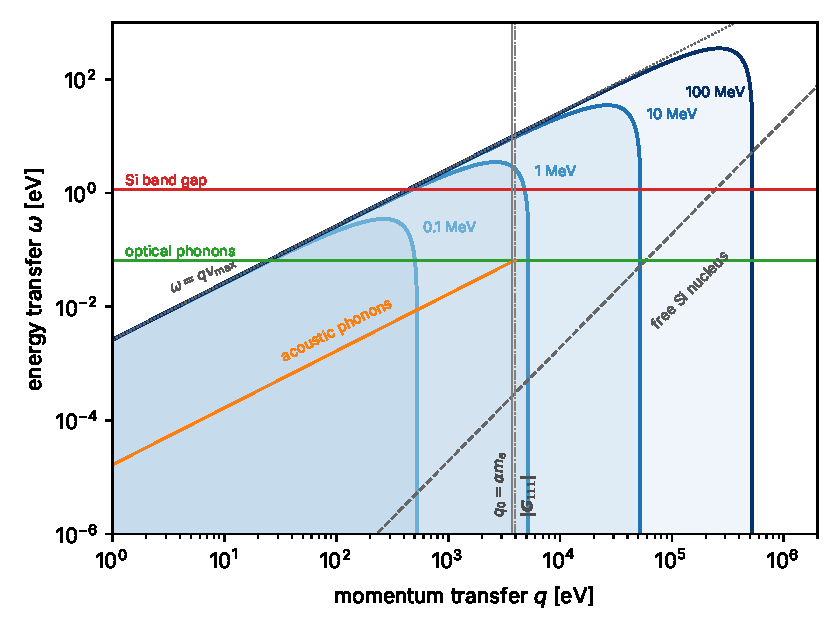
\includegraphics[width=0.9\linewidth]{figures/ch01/fig1_5.pdf}
  \caption{Momentum transfer $q$ and energy transfer $\omega$ accessible to elastic dark matter of mass 0.1, 1, 10 and \SI{100}{MeV} (blue curves, light to dark; shaded below), from $\omega \le qv_{\mathrm{max}} - q^2/2\mchi$ with $v_{\mathrm{max}} = \SI{794.5}{km.s^{-1}}$. The dotted line $\omega = qv_{\mathrm{max}}$ bounds all masses. Overlaid for silicon are the low-temperature band gap, \SI{1.17}{eV} (red), and the optical-phonon energy at the zone center, \SI{64}{meV} (green). The orange line is an acoustic branch $\omega$ = sound speed $\times\,q$ for a sound speed of \SI{5}{km.s^{-1}}, drawn up to $q = |\vect{G}_{111}|$, and the dashed curve is the recoil $q^2/2M$ of a free silicon nucleus, with $M = \SI{26.16}{GeV}$ the mean atomic mass of natural silicon. Vertical lines: the electron momentum scale $q_0 = \alpha m_e = \SI{3.73}{keV}$ and the length $|\vect{G}_{111}| = \sqrt{3}\,2\pi/a \approx \SI{4.0}{keV}$ of the shortest reciprocal-lattice vector of silicon, whose lattice constant is $a = 5.431$\,\AA. Scales from Refs.~\cites[Eqs.~(50) and (121), Sect.~IV\,A]{kahn2022searches}[Eq.~(11)]{ramanathan2020ionization}[lattice parameter of silicon]{mohr2025codata}.}
  \label{fig:1-kinematics}
\end{figure}

\begin{table}[tbp]
  \centering
  \caption{Kinematic extremes for elastic dark matter at $v_{\mathrm{max}} = \SI{794.5}{km.s^{-1}}$. Columns: the dark-matter mass; the largest momentum transfer to a target that absorbs any momentum; the largest energy transfer; the largest recoil energy of a free silicon nucleus ($M = \SI{26.16}{GeV}$, the mean atomic mass of natural silicon). The $\tfrac12\mchi v_{\mathrm{max}}^2$ column is also the threshold energy for which $m_{\mathrm{min}} = \mchi$.}
  \label{tab:1-kinematics}
  \begin{tabular}{@{}rrrr@{}}
    \toprule
    $\mchi$ & $2\mchi v_{\mathrm{max}}$ & $\tfrac12\mchi v_{\mathrm{max}}^2$ & free Si nucleus \\
    \midrule
    \SI{0.1}{MeV} & \SI{0.53}{keV} & \SI{0.35}{eV} & \SI{5.4}{\micro eV} \\
    \SI{1}{MeV} & \SI{5.3}{keV} & \SI{3.5}{eV} & \SI{0.54}{meV} \\
    \SI{10}{MeV} & \SI{53}{keV} & \SI{35}{eV} & \SI{54}{meV} \\
    \SI{100}{MeV} & \SI{530}{keV} & \SI{351}{eV} & \SI{5.3}{eV} \\
    \SI{1}{GeV} & \SI{5.3}{MeV} & \SI{3.5}{keV} & \SI{0.50}{keV} \\
    \bottomrule
  \end{tabular}
\end{table}

\Cref{fig:1-kinematics} answers at a glance which excitations each mass can reach. At \SI{0.1}{MeV} the largest deposit, \SI{0.35}{eV}, is below the silicon gap: only phonons, and other excitations below an eV, are open. At \SI{1}{MeV} the gap is open in a narrow band of momentum transfers, from $q = \SI{0.49}{keV}$ to \SI{4.8}{keV}, the two roots of \cref{eq:1.3-region} at $\omega = \SI{1.17}{eV}$. At \SI{10}{MeV} the band widens to 0.45--\SI{53}{keV}, and deposits up to \SI{35}{eV} are allowed. A free silicon nucleus, by contrast, receives \SI{1.17}{eV} only for $\mchi \gtrsim \SI{47}{MeV}$, where $2\mu_{\chi N}^2v_{\mathrm{max}}^2/M$ reaches that value.

Two momentum scales of the target, one for bound electrons and one for the lattice, decide what these momentum transfers probe. The first is the \emph{electron momentum scale}
\begin{equation}
  q_0 = \alpha m_e = \SI{3.73}{keV},
  \label{eq:1.3-q0}
\end{equation}
the inverse Bohr radius~\cite[Eq.~(121)]{kahn2022searches}. A bound outer electron has a wavefunction of size $1/(\alpha m_e)$ and typical momenta $\sim q_0$~\cite[Sect.~V\,A]{lin2019tasi}. A momentum transfer much smaller than $q_0$ barely changes the electron's state; a much larger one reaches only the high-momentum tail of its wavefunction. The second is the \emph{interatomic scale}, the length of the shortest reciprocal-lattice vector. For a cubic crystal with lattice constant $a$ the natural unit is $2\pi/a$. Silicon has $a = 5.431$\,\AA~\cite[lattice parameter of silicon]{mohr2025codata}, about ten Bohr radii~\cite[Sect.~V]{kahn2022searches}, which makes $2\pi/a = \SI{2.28}{keV} = 0.61\,q_0$. Its lattice is face-centered cubic, and the shortest reciprocal-lattice vectors, along the cube diagonals, are longer by $\sqrt{3}$: $|\vect{G}_{111}| = \sqrt{3}\,2\pi/a = \SI{3.95}{keV} \approx 1.06\,q_0$. A momentum transfer well below $|\vect{G}_{111}|$ has a wavelength longer than the interatomic spacing and sees the crystal as a whole; a larger one resolves the atoms. \Cref{sec:3.1} makes this precise with the reciprocal lattice.

The two scales are close to each other, and light dark matter straddles both. For an electronic excitation of a few eV, $q \ge \omega/v_{\mathrm{max}}$ requires $q \gtrsim \SI{1}{keV}$, roughly $0.3\,q_0$; the silicon gap alone needs $q \ge \SI{1.17}{eV}/2.650\times10^{-3} = \SI{0.44}{keV} = 0.12\,q_0$~\cite[Eq.~(123)]{kahn2022searches}. At the upper end, interpolating \cref{tab:1-kinematics}, $2\mchi v_{\mathrm{max}} = q_0$ at $\mchi = \SI{0.70}{MeV}$. Between about \SI{1}{MeV} and \SI{1}{GeV}, then, the momentum transfers match the momenta at which electrons in atoms and solids have most of their weight. Lighter dark matter cannot reach $q_0$ and probes the long-wavelength response of the crystal. Heavier dark matter can reach far above $q_0$, but momentum transfers of that size find little electronic weight.

The comparison with $|\vect{G}_{111}|$ explains why we never fold $\vect{q}$. Above about \SI{0.75}{MeV}, $2\mchi v_{\mathrm{max}}$ exceeds $|\vect{G}_{111}|$. Because the crystal conserves momentum only up to a reciprocal-lattice vector, the same excitation can be reached by momentum transfers that differ by such a vector, and these have different magnitudes. The dark-matter side, \cref{eq:1.3-omegaq,eq:1.3-vmin}, depends on the magnitude of the physical momentum transfer $\vect{q}$, not on its image in the first Brillouin zone. Folding $\vect{q}$ would assign the wrong $\vmin$ and the wrong dark-matter form factor $\FDM(q)$ of \cref{sec:1.4}. \Cref{sec:3.1} writes $\vect{q}$ as a first-zone part plus a reciprocal-lattice vector and keeps both.

On the energy side, electronic excitations and phonons set the scales. \emph{Electronic excitations} move an electron from an occupied to an empty state and typically cost an eV or more. In an insulator or semiconductor the lowest such energy is the \emph{band gap} $\Eg$ (\cref{we:1-mmin}; \cref{sec:3.3}). \emph{Phonons} are the quantized vibrations of the lattice, with energies from zero to roughly \SI{100}{meV}~\cite[Sect.~III\,A]{kahn2022searches}; the optical phonon of silicon at the zone center has \SI{64}{meV}, or \SI{15.5}{THz}~\cite{nilsson1972study} (\cref{sec:5.3}). Two kinds, optical and acoustic, matter here. Optical phonons, in which neighboring atoms move against each other, keep a finite energy as their momentum goes to zero. Acoustic phonons, long-wavelength sound waves, have energy equal to the sound speed times the momentum, with sound speeds of 3 to \SI{10}{km.s^{-1}}~\cite[Eq.~(50)]{kahn2022searches}, that is $1$ to $3\times10^{-5}$.

The kinematics treats optical and acoustic phonons differently. An optical phonon branch that is nearly flat, with energy $\omega$, can be excited at any $q$ between $\omega/v_{\mathrm{max}}$ and the upper root of \cref{eq:1.3-region}, close to $2\mchi v_{\mathrm{max}}$. Such a branch can absorb nearly the full kinetic energy, and \cref{eq:1.3-mmin} applies; the \SI{30}{meV} threshold of \cref{we:1-mmin} needs a momentum transfer of just $q \approx \SI{23}{eV}$, below a hundredth of $|\vect{G}_{111}|$. An acoustic phonon of branch $\nu$ has $\omega = c_\nu q$, with $c_\nu$ its sound speed (\cref{sec:5.2}). By \cref{eq:1.3-vmin} it needs $\vmin = c_\nu + q/2\mchi \le v$, which bounds $q \le 2\mchi(v - c_\nu)$ and $\omega \le 2c_\nu\mchi v$ to leading order in $c_\nu/v$~\cite[Eq.~(93)]{kahn2022searches}. The acoustic branch takes at most a fraction $4c_\nu/v$, a few percent, of the kinetic energy. In \cref{fig:1-kinematics} it is the orange line, which for the lightest mass leaves the parabola near its right end.

Both energy scales are material properties, and later chapters use computed values for them. The band gap is computed from first principles with density-functional theory, corrected for the systematic underestimate of gaps that the method makes (\cref{app:E.1,app:E.3}); phonon energies come from density-functional perturbation theory (\cref{app:E.4}). Measured values serve as checks.

\paragraph{Nuclear recoils.} \Cref{eq:1.3-ERmax} shows why scattering on free nuclei loses its reach for light dark matter. The free nucleus is the dashed parabola $\omega = q^2/2M$ of \cref{fig:1-kinematics}. It meets each dark-matter region only where $q^2/2M$ is small, because $M$ is large; for $\mchi \ll M$ the nucleus receives at most the fraction $4\mchi/M$ of the kinetic energy, $\num{1.5e-2}$ at \SI{100}{MeV} on silicon. The same parabola explains when a nucleus in a crystal is not free. A recoil energy comparable to the phonon energies, tens of meV, is reached at $\mchi \approx \SI{10}{MeV}$ (\cref{tab:1-kinematics}). Below that mass the nucleus cannot be treated as free: the dark matter excites one or a few phonons of the crystal instead, with the energies set by the lattice, and \cref{chap:5} develops that description.

For a free nucleus, \cref{eq:1.3-vmin} at $\omega = E_R = q^2/2M$ gives $\vmin = q/2\mu_{\chi N} = (ME_R/2\mu_{\chi N}^2)^{1/2}$. The crossover to phonons is already visible for a single nucleus held in a harmonic well of frequency $\omega_0$. At zero temperature a transfer $q$ excites $n$ quanta with the Poisson probability $P_n = \ee^{-E_R/\omega_0}(E_R/\omega_0)^n/n!$, where $E_R = q^2/2M$ is the free recoil energy~\cite[Eqs.~(90) and (91)]{kahn2022searches}. The energy deposit $n\omega_0$ therefore has mean exactly $E_R$ and rms spread $(E_R\omega_0)^{1/2}$. The free formula is the limit $E_R \gg \omega_0$, in which the spread is small compared with $E_R$.

\begin{limitbox}[Elastic nuclear recoil][lim:1.3a]
A free nucleus of mass $M$ at rest that receives momentum $q$ absorbs the energy $\omega = E_R = q^2/2M$. A dark-matter particle of speed $v$ gives it at most $E_R \le 2\mu_{\chi N}^2v^2/M$, with $\mu_{\chi N}$ the dark-matter--nucleus reduced mass, and a recoil $E_R$ needs the speed $v \ge \vmin = (ME_R/2\mu_{\chi N}^2)^{1/2}$~\cite[Eqs.~(77) and (78)]{lin2019tasi}.
\par\smallskip
{\centering
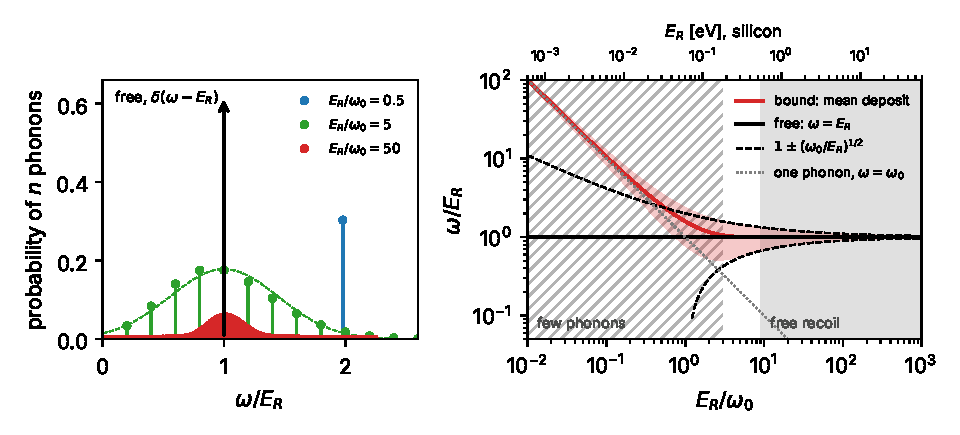
\includegraphics[width=\linewidth]{figures/ch01/limit1_nuclear.pdf}
\captionof{figure}{Free nuclear recoil against a nucleus bound in a harmonic (Einstein) potential of frequency $\omega_0 = \SI{60}{meV}$, a typical silicon phonon energy, at zero temperature~\cite[Sect.~IV\,A, Eqs.~(80), (90) and (91)]{kahn2022searches}. Left: probability of exciting $n$ phonons, a deposit $\omega = n\omega_0$, for $E_R/\omega_0 = 0.5$, 5 and 50 (dots; the term $n = 0$, which deposits nothing, is omitted), with Gaussians of rms width $(E_R\omega_0)^{1/2}$ (dashed) and the free response $\delta(\omega - E_R)$ (arrow). Right: mean deposit of the scatterings that excite the lattice (red line) and its rms spread (red band), against $E_R/\omega_0$, with the free value $\omega = E_R$ (black), the estimate $1 \pm (\omega_0/E_R)^{1/2}$ (dashed) and one phonon, $\omega = \omega_0$ (dotted); the top axis gives $E_R$ for silicon. Gray: $E_R \ge 9\omega_0 = \SI{0.54}{eV}$, where the rms width is below a third of $E_R$ and the free formula holds. Hatched: $E_R \le 3\omega_0$, the single- and few-phonon regime.}\label{fig:1-recoil-limit}
\par}
\smallskip
Below a few $\omega_0$ the deposit comes in whole phonons and spreads as widely as $E_R$ itself; below $\omega_0$ most scatterings leave the lattice unexcited, and the rest deposit at least one phonon, $\omega_0$, well above $E_R$.
\end{limitbox}

\begin{workedexample}{Largest recoil energy of a silicon nucleus}\label{we:1-nuclear}
For $\mchi = \SI{1}{GeV}$ on silicon, $M = \SI{26.16}{GeV}$ (the mean atomic mass of natural silicon) and $\mu_{\chi N} = (1 \times 26.16/27.16)\,\si{GeV} = \SI{0.963}{GeV}$. The maximum momentum transfer at $v_{\mathrm{max}}$ is $q = 2\mu_{\chi N}v_{\mathrm{max}} = 2 \times \SI{0.963}{GeV} \times 2.650\times10^{-3} = \SI{5.10}{MeV}$, and \cref{eq:1.3-ERmax} gives
\begin{equation*}
  E_R = \frac{q^2}{2M} = \frac{(\SI{5.10}{MeV})^2}{2 \times \SI{26160}{MeV}} = \SI{5.0e-4}{MeV} = \SI{0.50}{keV}.
\end{equation*}
The kinetic energy at $v_{\mathrm{max}}$ is $\tfrac12\mchi v_{\mathrm{max}}^2 = \SI{3.5}{keV}$, so the nucleus receives at most \SI{14}{\percent} of it; the exact fraction is $4\mu_{\chi N}^2/(\mchi M) = 0.142$. A typical particle, at $v \approx \SI{300}{km.s^{-1}}$ and with an average over angles, deposits far less. This momentum transfer, \SI{5.1}{MeV}, is below the inverse nuclear radius, tens of MeV, so the nucleus recoils coherently (\cref{sec:1.4}). On xenon, $M = \SI{122.3}{GeV}$, the same formula gives \SI{0.11}{keV}, the value quoted in \cref{sec:1.1}.
\end{workedexample}

\subsection{The speed integral}\label{sec:1.3-eta}

A rate sums the probability of each momentum transfer over the dark-matter velocities. Energy conservation enters it as a delta function $\delta(\omega - \omega_{\vect{q}})$, integrated against $f_\chi(\vect{v})$ (\cref{sec:2.2} derives the rate). The integral over $\vect{v}$ can be done once for all targets whose response depends on the magnitude $q$ but not on the direction of $\vect{q}$, as for a liquid, an atom, or a crystal averaged over orientations. For such a target only the angle $\theta$ between $\vect{q}$ and $\vect{v}$ matters. Its average is
\begin{equation*}
  \frac12\int_{-1}^{1} \dd(\cos\theta)\, \delta\!\left(\omega + \Delta_\chi + \frac{q^2}{2\mchi} - qv\cos\theta\right)
  = \frac{1}{2qv}\,\Theta\!\left(v - \vmin(q, \omega)\right).
\end{equation*}
The delta function fires once if its root $\cos\theta = (\omega + \Delta_\chi + q^2/2\mchi)/qv$ lies in $[-1, 1]$, which is the condition $v \ge \vmin$. The factor $1/qv$ is the derivative of its argument with respect to $\cos\theta$. This is the origin of the factor $1/v$ promised in \cref{sec:1.2}. Averaging over the halo, we find $\int \dd^3 v\, f_\chi(\vect{v})\,\Theta(v - \vmin)/(2qv) = \eta(\vmin)/(2q)$, with
\begin{equation}
  \eta(\vmin) \equiv \int \dd^3 v\, \frac{f_\chi(\vect{v})}{v}\,\Theta(v - \vmin) = \left\langle \frac{\Theta(v - \vmin)}{v}\right\rangle.
  \label{eq:1.3-eta}
\end{equation}
The function $\eta(\vmin)$ is the \emph{mean inverse speed above} $\vmin$. It carries all of the halo dependence of a rate for such a target~\cites[below Eq.~(5)]{essig2012direct}[Eqs.~(11) and (12)]{kahn2022searches}[Eqs.~(A.12)--(A.15)]{essig2016direct}. Its value at zero is the mean inverse speed $\langle 1/v\rangle$ of \cref{eq:1.2-inv}, and it decreases monotonically to zero at the largest speed in the halo. Because $\vmin \ge 0$ by \cref{eq:1.3-vmin}, $\eta$ is never needed at negative arguments.

\Cref{eq:1.3-eta} fixes how the halo enters the integral over momentum transfers. For an integrand that depends only on $q$, $\dd^3q/(2\pi)^3 = 4\pi q^2\dd q/(2\pi)^3$, and with the factor $\eta/2q$ the measure becomes~\cites[Eq.~(11)]{kahn2022searches}[Eq.~(A.14)]{essig2016direct}
\begin{equation*}
  \int\frac{\dd^3 q}{(2\pi)^3}\,\frac{\eta(\vmin)}{2q}\,(\cdots) = \int\frac{q\,\dd q}{4\pi^2}\,\eta\bigl(\vmin(q, \omega)\bigr)\,(\cdots).
\end{equation*}
Small momentum transfers carry the weight $q\,\dd q$, and $\eta$ cuts the integral off wherever $\vmin(q, \omega) > v_{\mathrm{max}}$, at both small and large $q$. \Cref{sec:1.5} assembles the full rate from this measure, the cross-section of \cref{sec:1.4} and the response of the target. For an anisotropic crystal at a fixed orientation the angular average does not factor out; the rate then depends on the direction of $\vect{v}_{\mathrm{E}}$ relative to the crystal axes, which is the daily modulation of \cref{sec:1.2}.

In the standard halo model the integral is elementary. With $F_\chi(v)$ the speed distribution of \cref{eq:1.2-Fspeed}, $\eta(\vmin) = \int_{\vmin}^\infty \dd v\, F_\chi(v)/v$, and the factor $v$ in $F_\chi$ cancels the $1/v$. \Cref{app:D.1} integrates the Gaussians and finds three branches in closed form: \cref{eq:D.1-eta1} for $0 \le \vmin < v_{\mathrm{esc}} - v_{\mathrm{E}}$, \cref{eq:D.1-eta2} for $v_{\mathrm{esc}} - v_{\mathrm{E}} \le \vmin < v_{\mathrm{esc}} + v_{\mathrm{E}}$, and $\eta = 0$ above. Both are differences of error functions (\cref{app:C.8}) minus a constant from the cut, with $v_{\mathrm{E}} = |\vect{v}_{\mathrm{E}}(t)|$.

\Cref{fig:1-eta} shows $\eta$ at the reference Earth speed and on the days of largest and smallest Earth speed. Three features matter for light dark matter: a plateau, a Gaussian fall and a second branch. Up to $\vmin \approx \SI{200}{km.s^{-1}}$, $\eta$ stays within a factor of 1.41 of $\langle 1/v\rangle = 1/(\SI{287.9}{km.s^{-1}})$: almost every particle qualifies. Between 300 and \SI{700}{km.s^{-1}} it falls roughly as a Gaussian, $\ee^{-(\vmin - v_{\mathrm{E}})^2/v_0^2}$, by a factor of 190, from \SI{1.53e-3}{(km/s)^{-1}} to \SI{7.95e-6}{(km/s)^{-1}}. Above $v_{\mathrm{esc}} - v_{\mathrm{E}}^{\mathrm{ref}} = \SI{293.5}{km.s^{-1}}$ the second branch applies; every $\vmin$ near a kinematic threshold lies on it. In natural units, $\eta(0) = 1041$, $\eta(\SI{600}{km.s^{-1}}) = 19.2$ and $\eta(\SI{700}{km.s^{-1}}) = 2.38$.

\begin{figure}[tbp]
  \centering
  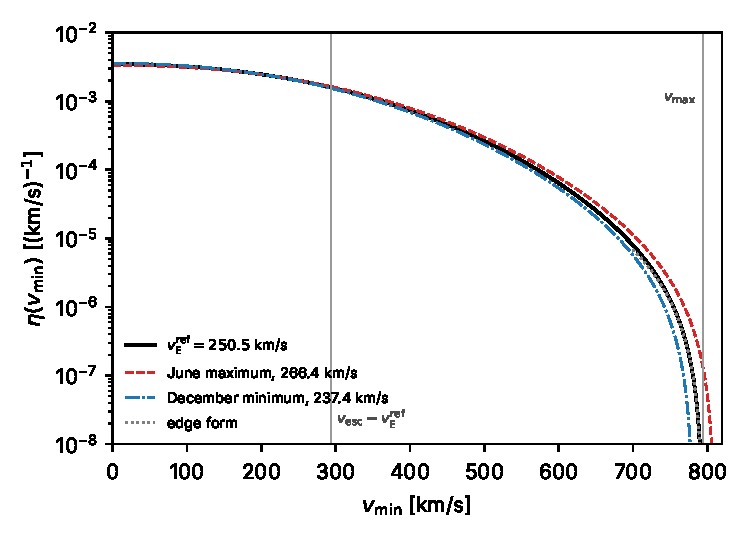
\includegraphics[width=0.8\linewidth]{figures/ch01/fig1_6.pdf}
  \caption{Mean inverse speed above $\vmin$, $\eta(\vmin) = \langle\Theta(v - \vmin)/v\rangle$, in the standard halo model ($v_0 = \SI{238}{km.s^{-1}}$, $v_{\mathrm{esc}} = \SI{544}{km.s^{-1}}$). Solid: Earth speed $v_{\mathrm{E}}^{\mathrm{ref}} = \SI{250.5}{km.s^{-1}}$; dashed: June maximum (\SI{266.4}{km.s^{-1}}); dash-dotted: December minimum (\SI{237.4}{km.s^{-1}}). Vertical lines: $v_{\mathrm{esc}} - v_{\mathrm{E}}^{\mathrm{ref}} = \SI{293.5}{km.s^{-1}}$, where the closed form changes branch, and $v_{\mathrm{max}} = \SI{794.5}{km.s^{-1}}$, where $\eta$ vanishes. The dotted curve above \SI{700}{km.s^{-1}} is the edge form of \cref{eq:1.3-edge} with its first correction; it lies within \SI{10}{\percent} of the exact curve above \SI{720}{km.s^{-1}}, within \SI{5}{\percent} above \SI{745}{km.s^{-1}}, and merges with it toward $v_{\mathrm{max}}$. At $\vmin = 0$, $\eta = 1/(\SI{287.9}{km.s^{-1}})$, or 1041 in natural units. Closed form from \cref{app:D.1}; halo parameters from Ref.~\cite[Table~1]{baxter2021recommended}.}
  \label{fig:1-eta}
\end{figure}

Near the end point the moving cut dominates the seasonal change. Relative to the reference curve, $\eta$ in June and December is 1.42 and 0.72 times as large at $\vmin = \SI{700}{km.s^{-1}}$, 2.2 and 0.37 times at \SI{760}{km.s^{-1}}, and 4.5 and 0.009 times at \SI{780}{km.s^{-1}}, where the December halo has almost no particles left.

\subsection{The kinematic edge}\label{sec:1.3-edge}

The \emph{kinematic edge} of a rate is the boundary beyond which no particle in the halo is fast enough. At fixed $\mchi$ the spectrum ends at $\omega = \tfrac12\mchi v_{\mathrm{max}}^2 - \Delta_\chi$, by \cref{eq:1.3-omegamax}. At a fixed threshold the rate, as a function of mass, ends at $m_{\mathrm{min}}$. Both edges are reached as $\vmin \to v_{\mathrm{max}}$, and the shape of a rate near an edge is controlled by the shape of $\eta$ there.

Close to $v_{\mathrm{max}}$, $\eta$ vanishes as a power. Write $\vmin = v_{\mathrm{esc}} + v_{\mathrm{E}} - \delta$ with small $\delta > 0$. On the second branch, \cref{eq:D.1-eta2}, the difference of error functions is an integral, $(\sqrt{\pi}v_0/2)[\operatorname{erf}(v_{\mathrm{esc}}/v_0) - \operatorname{erf}((v_{\mathrm{esc}} - \delta)/v_0)] = \int_{v_{\mathrm{esc}} - \delta}^{v_{\mathrm{esc}}}\ee^{-y^2/v_0^2}\dd y$, and the constant term is $\delta\,\ee^{-v_{\mathrm{esc}}^2/v_0^2} = \int_{v_{\mathrm{esc}} - \delta}^{v_{\mathrm{esc}}}\ee^{-v_{\mathrm{esc}}^2/v_0^2}\dd y$. With $s = v_{\mathrm{esc}} - y$, the integrand of their difference is
\begin{equation*}
  \ee^{-v_{\mathrm{esc}}^2/v_0^2}\left[\ee^{(2v_{\mathrm{esc}}s - s^2)/v_0^2} - 1\right]
  = \ee^{-v_{\mathrm{esc}}^2/v_0^2}\left[\frac{2v_{\mathrm{esc}}s}{v_0^2} + \left(\frac{2v_{\mathrm{esc}}^2}{v_0^4} - \frac{1}{v_0^2}\right)s^2 + O(s^3)\right].
\end{equation*}
Integrating over $0 < s < \delta$ and multiplying by the prefactor $\pi v_0^2/(v_{\mathrm{E}}N_{\mathrm{esc}})$,
\begin{equation}
  \eta(\vmin) = \frac{\pi v_{\mathrm{esc}}\,\ee^{-v_{\mathrm{esc}}^2/v_0^2}}{v_{\mathrm{E}}N_{\mathrm{esc}}}\,\delta^2\left[1 + \frac{(2v_{\mathrm{esc}}^2 - v_0^2)\,\delta}{3v_{\mathrm{esc}}v_0^2} + O(\delta^2)\right],
  \qquad \delta = v_{\mathrm{esc}} + v_{\mathrm{E}} - \vmin .
  \label{eq:1.3-edge}
\end{equation}
The scale of the correction is $3v_{\mathrm{esc}}v_0^2/(2v_{\mathrm{esc}}^2 - v_0^2) = \SI{173}{km.s^{-1}}$. At the reference Earth speed and $\vmin = 760$ and \SI{780}{km.s^{-1}} ($\delta = 34.5$ and \SI{14.5}{km.s^{-1}}), the quadratic term alone captures 0.81 and 0.92 of the exact value, and with the correction 0.98 and 1.00. The edge is quadratic because two things vanish together: the speed window $v_{\mathrm{max}} - \vmin$, and the density of particles inside it, which drops linearly to zero at the escape speed of the truncated Maxwellian. The prefactor $\ee^{-v_{\mathrm{esc}}^2/v_0^2}/N_{\mathrm{esc}}$ is the height of the distribution at the cut. Both factors are fixed by the most uncertain parts of the halo model (\cref{sec:1.2}); a smoother truncation would raise the power of $\delta$.

The edge in mass follows. For a threshold $E_{\mathrm{th}}$ the smallest $\vmin$ available to a particle of mass $\mchi$ is $(2E_{\mathrm{th}}/\mchi)^{1/2}$ (below \cref{eq:1.3-omegamax}). Its distance from $v_{\mathrm{max}}$ is
\begin{equation*}
  v_{\mathrm{max}} - \left(\frac{2E_{\mathrm{th}}}{\mchi}\right)^{1/2} = v_{\mathrm{max}}\left[1 - \left(\frac{m_{\mathrm{min}}}{\mchi}\right)^{1/2}\right] \simeq \frac{v_{\mathrm{max}}}{2}\,\frac{\mchi - m_{\mathrm{min}}}{m_{\mathrm{min}}},
\end{equation*}
so a mass one percent above $m_{\mathrm{min}}$ uses only particles within \SI{4}{km.s^{-1}} of $v_{\mathrm{max}}$. Just above the edge the rate is the product of $\eta$, quadratic in this window, and of the phase space of pairs $(q, \omega)$ that fit inside it, which shrinks as a further power of the window. How fast that phase space shrinks depends on how the target's response begins at threshold. For silicon the electronic response begins at a crystal momentum away from the zone center, and the question becomes which excitations the dark matter can reach at the edge (\cref{sec:3.3}).

The recovery above the edge is slow. Take the silicon gap of \cref{we:1-mmin} as threshold, $m_{\mathrm{min}} = \SI{0.333}{MeV}$, and evaluate $\eta$ at the most favorable speed $(2\Eg/\mchi)^{1/2}$, an upper bound on what the halo offers at each mass. Relative to $\eta(0)$, it is $\num{6.0e-5}$ at \SI{0.35}{MeV}, $\num{1.1e-3}$ at \SI{0.4}{MeV}, \SI{0.76}{\percent} at \SI{0.5}{MeV}, \SI{12}{\percent} at \SI{1}{MeV} and \SI{84}{\percent} at \SI{10}{MeV}. Between \SI{0.35}{MeV}, \SI{5}{\percent} above $m_{\mathrm{min}}$, and $2m_{\mathrm{min}}$ the halo supply grows by a factor of more than 500. The whole of that range is set by particles faster than about \SI{560}{km.s^{-1}}, the most favorable speed at $2m_{\mathrm{min}}$, which are \SI{7}{\percent} of the halo. A limit in this mass range is a statement about the tail of the velocity distribution as much as about the target.

The position of the edge, by contrast, depends on the target and the halo only through $E_{\mathrm{th}}/v_{\mathrm{max}}^2$. Their uncertainties enter as $\delta\ln m_{\mathrm{min}} = \delta\ln E_{\mathrm{th}} - 2\,\delta\ln v_{\mathrm{max}}$. A \SI{5}{\percent} change in the gap moves $m_{\mathrm{min}}$ by \SI{5}{\percent}.

\section{Light dark-matter models}\label{sec:1.4}

Kinematics (\cref{sec:1.3}) decides which pairs $(\vect{q}, \omega)$ are open; the interaction with electrons and nuclei decides how often they occur. Model building itself is covered by reviews~\cites[Sect.~III]{lin2019tasi}{kahn2022searches}; we keep only what fixes a rate.

\subsection{Mediators and the Yukawa potential}

Thermal light dark matter needs a mediator with a mass at or below the GeV scale (\cref{sec:1.1}). We take it to be either a massive vector field $A'_\mu$ or a real scalar field $\phi_V$, with mass $m_V$ and couplings $y_\chi$ to dark matter, $y_e$ to electrons and $y_N$ to nucleons. The vector couples to a current of each species and the scalar to a density ($\bar\psi\gamma^\mu\psi$ and $\bar\psi\psi$ in field-theory notation). For slow particles both reduce, at leading order, to the number density~\cite[Eq.~(7)]{knapen2021dark}, and we use only that limit. The interaction Lagrangian densities are then
\begin{equation}
  \mathcal{L}_{\mathrm{int}} = -A'_\mu\bigl(y_\chi J^\mu_\chi + y_e J^\mu_e + y_N J^\mu_N\bigr)
  \quad\text{or}\quad
  \mathcal{L}_{\mathrm{int}} = -\phi_V\bigl(y_\chi \nd_\chi + y_e \nd_e + y_N \nd_N\bigr),
  \label{eq:1.4-Lint}
\end{equation}
where $J^\mu_\chi$, $J^\mu_e$ and $J^\mu_N$ are number currents whose time components are the number densities $\nd_\chi$, $\nd_e$ and $\nd_N$. The spatial components carry a factor of the particle velocity; they lead to velocity-dependent interactions, mentioned at the end of this section, and do not enter the potential below.

The mediator can be treated as a classical field sourced by the particles. A dark-matter particle at rest at the origin is a point source $y_\chi\delta^3(\vect{x})$. For this static source the Euler--Lagrange equation of the vector field reduces to the static Klein--Gordon equation $(-\nabla^2 + m_V^2)A'^0 = y_\chi\delta^3(\vect{x})$ (\cref{eq:C.9-static}). Its solution is $y_\chi$ times the Green's function of \cref{eq:C.9-Gx}, $A'^0(\vect{x}) = y_\chi\,\ee^{-m_V r}/(4\pi r)$ with $r = |\vect{x}|$. By \cref{eq:1.4-Lint}, an electron at $\vect{x}$ has the potential energy $y_e A'^0(\vect{x})$. The dark-matter--electron potential is then
\begin{equation}
  V(\vect{x}) = y_\chi y_e\,\frac{\ee^{-m_V|\vect{x}|}}{4\pi|\vect{x}|},
  \label{eq:1.4-yukawa}
\end{equation}
the Yukawa potential. It has range $1/m_V$ and becomes Coulomb-like as $m_V \to 0$. A scalar mediator leads to the same function with the opposite sign: vector exchange repels sources whose couplings have equal signs, and scalar exchange attracts them (\cref{eq:C.9-U}, where the signs are derived from the field energy). With the Fourier convention of \cref{app:A.3} and \cref{eq:C.9-Gq}, the transform is
\begin{keyresult}[Yukawa potential in momentum space]
\begin{equation}
  \tilde V(\vect{q}) = \int\dd^3x\,\ee^{+\ii\vect{q}\cdot\vect{x}}\,V(\vect{x}) = \frac{y_\chi y_e}{q^2 + m_V^2}.
  \label{eq:1.4-Vq}
\end{equation}
For a scalar mediator the sign is reversed. Since every rate in this book depends on $|\tilde V(\vect{q})|^2$, the sign does not enter.
\end{keyresult}

\noindent Here $\vect{q}$ is the momentum the dark matter transfers to the target (\cref{sec:1.3}). Because $V(\vect{x})$ depends only on the separation, the amplitude for transferring $\vect{q}$ is proportional to $\tilde V(\vect{q})$ (\cref{app:C.9}; derived in \cref{sec:2.2}). \Cref{eq:1.4-Vq} has two limits, which the field calls the heavy- and light-mediator limits. For a heavy mediator, with $m_V$ above every relevant $q$, $\tilde V$ is a constant: a contact interaction. For a light mediator, with $m_V$ below every relevant $q$, $\tilde V \propto 1/q^2$, as in Coulomb scattering. The potential is static because the energy deposited is small: a moving source adds $-\omega^2$ to $q^2 + m_V^2$ in the denominator, and in scattering $\omega \le qv$ with $v \lesssim 3\times10^{-3}$, which keeps the correction below $10^{-5}$ (\cref{app:C.9}).

Which couplings a mediator has depends on the model. A vector coupled to electric charge, the dark photon below, couples to electrons and protons and not to neutrons. A vector coupled to baryon minus lepton number couples to electrons, protons and neutrons with equal magnitude. A scalar that mixes with the Higgs boson couples to each fermion in proportion to its mass, which makes $y_N/y_e$ large~\cite[Sect.~III\,C]{lin2019tasi}. Each mediator is constrained by accelerator, stellar and cosmological data, which bound the products $y_\chi y_e$ and $y_\chi y_N$ that enter rates and the couplings to ordinary matter separately~\cite[Sect.~III\,C]{lin2019tasi}. We will not need these bounds, since the rates below depend on the models only through $\tilde V(\vect{q})$ and the absorption couplings.

\subsection{Reference cross-section and form factor}

Experiments compare models through the reference cross-section $\sigmae$ and the dark-matter form factor $\FDM(q)$, both fixed by $\tilde V(\vect{q})$. The reference momentum is $q_0 = \alpha m_e = \SI{3.73}{keV}$ (\cref{sec:1.3}), the inverse Bohr radius, typical of electrons bound in atoms and solids. We define~\cites[Eqs.~(3) and (4)]{essig2012direct}[Eqs.~(11) and (12)]{knapen2021dark}
\begin{equation}
  \sigmae \equiv \frac{\mu_{\chi e}^2}{\pi}\,|\tilde V(q_0)|^2,
  \qquad
  \FDM(q) \equiv \frac{\tilde V(q)}{\tilde V(q_0)},
  \label{eq:1.4-defs}
\end{equation}
with $\mu_{\chi e}$ the dark-matter--electron reduced mass (\cref{sec:1.3}). Equivalently,
\begin{equation}
  |\tilde V(q)|^2 = \frac{\pi\sigmae}{\mu_{\chi e}^2}\,\FDM(q)^2 ,
  \label{eq:1.4-Vsq}
\end{equation}
the form in which the interaction enters every electron-scattering rate in this book. For the Yukawa potential of \cref{eq:1.4-Vq},
\begin{equation}
  \sigmae = \frac{\mu_{\chi e}^2\, y_\chi^2 y_e^2}{\pi\,(m_V^2 + \alpha^2 m_e^2)^2},
  \qquad
  \FDM(q) = \frac{m_V^2 + \alpha^2 m_e^2}{m_V^2 + q^2},
  \label{eq:1.4-yukawa-sigma}
\end{equation}
in agreement with Ref.~\cite[Eqs.~(11) and (12)]{knapen2021dark}.

Which process does $\sigmae$ describe? For a potential whose transform is a constant $\tilde V$, the first Born approximation yields the free elastic cross-section $\mu_{\chi e}^2|\tilde V|^2/\pi$ (\cref{app:C.9}; derived in \cref{sec:2.2}). It is that cross-section with $\tilde V$ frozen at $q_0$; for a heavy mediator it is the actual cross-section of dark matter on a free electron. For a light mediator, however, it is the cross-section of no process: the free cross-section of a $1/q^2$ potential diverges at small angles, as Rutherford's does, and $\sigmae$ merely normalizes $|\tilde V(q_0)|^2$. In a target the divergence is cut off by the minimum momentum transfer needed to excite it and by screening. Since $\sigmae$ is defined in vacuum, with screening and every other in-medium effect assigned to the target response (\cref{sec:4.4}), a quoted $\sigmae$ means the same thing for every target. Other papers use other reference points and normalizations (\cref{app:A.9}).

Two limits of \cref{eq:1.4-yukawa-sigma} cover most of the literature. A heavy mediator, $m_V$ above both $q_0$ and every momentum transfer that contributes, gives $\FDM = 1$ and $\sigmae = \mu_{\chi e}^2 y_\chi^2 y_e^2/(\pi m_V^4)$. A light mediator, $m_V$ below both, gives $\FDM = (q_0/q)^2$ and $\sigmae = \mu_{\chi e}^2 y_\chi^2 y_e^2/(\pi q_0^4)$. To first order in the small ratio, $\FDM \simeq 1 + (q_0^2 - q^2)/m_V^2$ for the heavy mediator and $\FDM \simeq (q_0/q)^2\,(1 + m_V^2/q_0^2 - m_V^2/q^2)$ for the light one. The momentum transfers that contribute run from $\omega/v_{\mathrm{max}}$, \SI{0.44}{keV} $= 0.12\,q_0$ for the silicon gap, up to $2m_\chi v_{\mathrm{max}}$ (\cref{sec:1.3}).

\begin{limitbox}[Heavy and light mediators][lim:1.4a]
For a mediator of mass $m_V$ and a momentum transfer $q$, the form factor of \cref{eq:1.4-defs} is $\FDM(q) = 1$ when $m_V \gg q, q_0$ (heavy mediator) and $\FDM(q) = (q_0/q)^2$ when $m_V \ll q, q_0$ (light mediator), with $q_0 = \alpha m_e$~\cite[Eq.~(15) and the display above it]{essig2012direct}.
\par\smallskip
{\centering
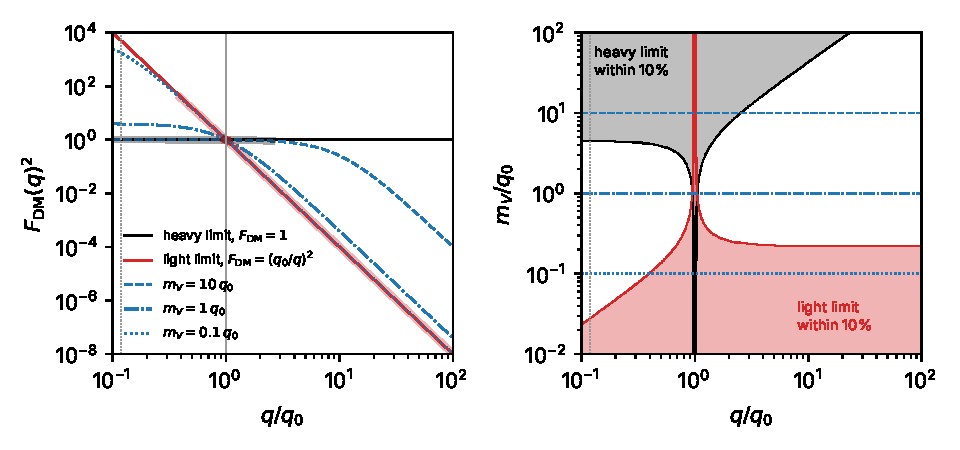
\includegraphics[width=\linewidth]{figures/ch01/fig1_7.pdf}
\captionof{figure}{Squared dark-matter form factor $\FDM(q)^2 = [(m_V^2 + q_0^2)/(m_V^2 + q^2)]^2$~\cite[Eq.~(12)]{knapen2021dark}, with $q_0 = \alpha m_e = \SI{3.73}{keV}$. Left: $\FDM^2$ against $q/q_0$ for $m_V = 10\,q_0$ (dashed), $q_0$ (dash-dotted) and $0.1\,q_0$ (dotted), between the heavy limit $\FDM = 1$ (black) and the light limit $(q_0/q)^4$ (red). A curve is overdrawn in gray or light red where it lies within \SI{10}{\percent} of the heavy or light limit, $|\FDM^2/\text{limit} - 1| \le 0.1$. Right: the same two regions in the plane of $q/q_0$ and $m_V/q_0$; the horizontal lines are the three mediator masses of the left panel. Every curve equals both limits at $q = q_0$ by construction, which produces the narrow vertical strip. Dotted vertical line: $q = 0.12\,q_0$, the smallest momentum transfer that crosses the low-temperature silicon gap. Across $0.12\,q_0 \le q \le q_0$ the heavy limit holds for $m_V \ge 4.5\,q_0 = \SI{17}{keV}$; for all $q \ge 0.12\,q_0$ the light limit holds for $m_V \le 0.028\,q_0 = \SI{0.10}{keV}$.}\label{fig:1-fdm}
\par}
\smallskip
For $m_V$ within a factor of a few of the momentum transfers that the target samples, neither limit holds, and rates must use the full form of \cref{eq:1.4-yukawa-sigma}.
\end{limitbox}

A light mediator weights the rate toward small momentum transfers, by $(q_0/q)^4$, and favors excitations near the kinematic threshold at small $q$, which is also where the target screens most strongly (\cref{sec:4.4}).

\subsection{The dark photon}

The most studied vector mediator is the dark photon: the gauge boson of a new U(1) symmetry under which the dark matter carries charge $y_\chi$ and ordinary matter carries none. It reaches ordinary matter through kinetic mixing, a term $(\zeta/2)F_{\mu\nu}F'^{\mu\nu}$ that couples the photon field strength $F_{\mu\nu}$ to its own, $F'_{\mu\nu}$, with a dimensionless strength $\zeta$~\cite{holdom1986two}. The literature writes $\epsilon$, $\kappa$ or $\chi$ for $\zeta$ (\cref{app:B.2}). Gauge invariance permits the term, and loops of heavy particles charged under both symmetries generate it~\cite{holdom1986two}. The mixing is removed by shifting the photon field, $A_\mu = \tilde A_\mu + \zeta A'_\mu$, which leaves the mass term of $A'_\mu$ unchanged (\cref{eq:C.9-mix,eq:C.9-mixed}).

\begin{keyresult}[Dark-photon couplings]
To first order in $\zeta$, the massive dark photon $A'_\mu$ couples to the dark-matter current with strength $y_\chi$ and to the electromagnetic current $J^\mu_{\mathrm{em}}$ with strength $\zeta e$, through $\mathcal{L} \supset -\zeta e\,A'_\mu J^\mu_{\mathrm{em}} - y_\chi A'_\mu J^\mu_\chi$. Here $e > 0$ is the elementary charge, $e^2 = 4\pi\alpha$ (\cref{app:A.2}), and $J^\mu_{\mathrm{em}}$ counts each particle with its charge in units of $e$. In the notation of \cref{eq:1.4-Lint} the electron coupling is $y_e = -\zeta e$, since the electron charge is $-e$; protons have $+\zeta e$ and neutrons zero. The dark matter stays neutral under the photon.
\end{keyresult}

\noindent Inserting $y_e^2 = 4\pi\alpha\zeta^2$ into \cref{eq:1.4-yukawa-sigma}, we find~\cite[Eq.~(74)]{lin2019tasi}
\begin{equation}
  \sigmae = \frac{4\alpha\,\zeta^2 y_\chi^2\,\mu_{\chi e}^2}{(m_V^2 + \alpha^2 m_e^2)^2}.
  \label{eq:1.4-darkphoton}
\end{equation}
Ref.~\cite[display above Eq.~(15)]{essig2012direct} writes it with $y_\chi^2 = 4\pi\alpha_D$, where $\alpha_D$ is a dark fine-structure constant.

\begin{workedexample}{Reference cross-section of a heavy dark photon}\label{we:1-darkphoton}
We take the thermal-relic benchmark of Ref.~\cite[Sect.~III\,D]{lin2019tasi}: $m_\chi = \SI{10}{MeV}$, $m_V = \SI{30}{MeV}$, $y_\chi = 0.3$ and $\zeta = 10^{-4}$. The reduced mass is $\mu_{\chi e} = m_e m_\chi/(m_e + m_\chi) = (0.511 \times 10/10.511)\,\si{MeV} = \SI{0.486}{MeV}$, so $\mu_{\chi e}^2 = \SI{0.236}{MeV^2}$. The maximum momentum transfer is $2m_\chi v_{\mathrm{max}} = \SI{0.053}{MeV}$, smaller than $m_V$ by a factor of 570: the mediator is heavy, $\FDM = 1$, and $\alpha^2 m_e^2/m_V^2 = 1.5\times10^{-8}$ can be dropped in \cref{eq:1.4-darkphoton}. With $4\alpha = 0.0292$, $\zeta^2 = 10^{-8}$ and $y_\chi^2 = 0.09$,
\begin{equation*}
  \begin{aligned}
  \sigmae &= \frac{4\alpha\,\zeta^2 y_\chi^2\,\mu_{\chi e}^2}{m_V^4}
  = \frac{0.0292 \times 10^{-8} \times 0.09 \times \SI{0.236}{MeV^2}}{(\SI{30}{MeV})^4} \\
  &= \frac{\SI{6.21e-12}{MeV^2}}{\SI{8.10e5}{MeV^4}} = \SI{7.67e-18}{MeV^{-2}}
  \end{aligned}.
\end{equation*}
With $(\hbar c)^2 = \SI{3.894e-22}{MeV^2.cm^2}$ this is $\sigmae = \SI{3.0e-39}{cm^2}$. Ref.~\cite[Sect.~III\,D]{lin2019tasi} quotes about \SI{e-37}{cm^2} for both of its benchmarks, although its own Eq.~(74) leads to the value found here for this one. At fixed couplings $\sigmae$ scales as $m_V^{-4}$, and for $m_\chi \gg m_e$ it hardly depends on $m_\chi$, because $\mu_{\chi e} \to m_e$.
\end{workedexample}

Freeze-out and freeze-in, the two production histories of \cref{sec:1.1}, lead to the heavy- and light-mediator limits of the form factor. Thermal freeze-out through a dark photon needs couplings large enough to deplete the dark matter, which favors a heavy mediator as in \cref{we:1-darkphoton}. Freeze-in, by contrast, needs couplings so feeble that the dark matter never reaches equilibrium; with an ultralight dark photon the rate of scattering on electrons is still observable, because the light-mediator limit enhances small momentum transfers. The freeze-in benchmark of Ref.~\cite[Sect.~III\,D]{lin2019tasi}, $m_\chi = \SI{1}{MeV}$, $m_V = \SI{e-12}{eV}$, $y_\chi = 3\times10^{-6}$ and $\zeta = 10^{-6}$, has $\FDM = (q_0/q)^2$ and, from the light limit of \cref{eq:1.4-darkphoton} with $\mu_{\chi e} = \SI{0.338}{MeV}$, $\sigmae = 4\alpha\zeta^2 y_\chi^2\mu_{\chi e}^2/q_0^4 = \SI{6.1e-38}{cm^2}$.

The field redefinition holds in vacuum. In a medium the photon has a self-energy $\Pi_{\mathrm{em}}$ from the charges it polarizes, and the medium modifies the mixing. For absorption of a dark photon at rest, with $\omega = m_V$ and $q \to 0$, the effective mixing is $\zeta_{\mathrm{eff}}^2 = \zeta^2 m_V^4/\{[m_V^2 - \Real\Pi_{\mathrm{em}}(m_V)]^2 + [\Imag\Pi_{\mathrm{em}}(m_V)]^2\}$~\cite[Eqs.~(5) and (6), with $\kappa$ for $\zeta$]{hochberg2017absorption}. It is suppressed where $m_V$ lies below the scale of $|\Pi_{\mathrm{em}}|$, which in metals and semiconductors is set by the plasma frequency (\cref{sec:4.3}), and approaches $\zeta$ well above it. For scattering, the same physics is the screening of the dark photon's potential by the target. In the convention of this section, where $\tilde V(\vect{q})$ is the unscreened potential, the screening is a factor $1/|\varepsilon(\vect{q}, \omega)|^2$ inside the target response~\cite[Eqs.~(6) and (8)]{knapen2021dark}, and $\sigmae$ stays a vacuum quantity. The self-energy $\Pi_{\mathrm{em}}$ and the longitudinal dielectric function $\varepsilon(\vect{q}, \omega)$ are material quantities: they are measured optically or computed from first principles, in the random-phase approximation with local fields or in time-dependent density-functional theory (\cref{app:E.6}). \Cref{sec:4.4} treats screening, and \cref{chap:10} the in-medium dark photon.

\subsection{Scattering on nuclei}

A mediator that couples to nucleons with strength $y_N$, the same for protons and neutrons, leads to a dark-matter--nucleon potential of the form of \cref{eq:1.4-Vq} with $y_e \to y_N$. For a heavy mediator the dark-matter--proton cross-section is $\sigma_p = \mu_{\chi p}^2 y_\chi^2 y_N^2/(\pi m_V^4)$~\cite[Eq.~(99)]{lin2019tasi}, the analogue of $\sigmae$, with $\mu_{\chi p}$ the dark-matter--proton reduced mass. A nucleus of mass number $A$ and atomic number $Z$ holds $A$ nucleons within a radius of a few fm. When $q$ is small compared with the inverse nuclear radius, $1/R \approx \SI{57}{MeV}$ for silicon, whose nuclear radius is $R \approx \SI{3.47}{fm}$ (\cref{sec:2.2}), the phase $\ee^{\ii\vect{q}\cdot\vect{x}}$ is the same for every nucleon, and the Fourier transform of the summed potential is $A$ times the single-nucleon transform. The amplitudes add coherently.

Replacing $y_N$ by $Ay_N$ and $\mu_{\chi p}$ by the dark-matter--nucleus reduced mass $\mu_{\chi N}$ in $\sigma_p$ gives
\begin{equation}
  \sigma_N = \sigma_p\left(\frac{\mu_{\chi N}}{\mu_{\chi p}}\right)^2 A^2 ,
  \label{eq:1.4-sigmaN}
\end{equation}
the standard convention for spin-independent scattering~\cites{lewin1996review}[Eq.~(104)]{lin2019tasi}. If protons and neutrons couple differently, $A$ becomes $Z + (A - Z)y_n/y_p$, with $y_p$ and $y_n$ the two couplings~\cite[Eq.~(104)]{lin2019tasi}. Since a dark photon couples only to charge, $A^2$ becomes $Z^2$ for it. For silicon, $A = 28$ and $Z = 14$, with the mean atomic mass of natural silicon, \SI{26.16}{GeV}. \Cref{we:2-coherent} evaluates $\sigma_N/\sigma_p$ for silicon.

At larger $q$ the nuclear form factor $F_{\mathrm{Helm}}(q)$ of \cref{sec:2.2} multiplies the amplitude. For the light dark matter of this book the momentum transfer stays below $2m_\chi v_{\mathrm{max}} \approx \SI{5}{MeV}$ even at $m_\chi = \SI{1}{GeV}$, and the nucleus is always coherent. At $q$ below the inverse size of an atom, the electrons screen the nuclear charge seen by a dark photon; this enters through the target response (\cref{sec:4.4}). In a crystal, however, the nuclei are bound, and at low $q$ the dark matter excites phonons instead of free recoils (\cref{chap:5}).

\subsection{Absorption of bosonic dark matter}

Dark matter lighter than about a keV cannot be a thermal relic (\cref{sec:1.1}), but bosons in this range can be produced non-thermally, for example by misalignment, and behave as a classical field oscillating at their mass~\cite[Sect.~I\,B]{lin2019tasi}. Such a boson $\phi$ of mass $m_\phi$ can be absorbed: it disappears and deposits its whole energy in the target. Bound to the Galaxy, it moves at $v \approx 10^{-3}$ and carries energy $m_\phi(1 + v^2/2) \approx m_\phi$ and momentum $\vect{p}_\phi = m_\phi\vect{v}$. Absorption then deposits
\begin{equation}
  \omega \approx m_\phi, \qquad \vect{q} = \vect{p}_\phi, \qquad |\vect{p}_\phi| \approx m_\phi v \approx 10^{-3}\,\omega .
  \label{eq:1.4-absorption}
\end{equation}
The momentum is much smaller than the energy, the reverse of scattering, where $\omega \le qv$ (\cref{sec:1.3}). Absorption probes the response of the target at $q \to 0$, the regime of optical absorption, at a single energy, $\omega = m_\phi$. Compared to scattering, absorption also reaches lower masses. A scattering particle can deposit at most its kinetic energy, and crossing a gap $\Eg$ needs $m_\chi \ge 2\Eg/v_{\mathrm{max}}^2$ (\cref{sec:1.3}), about \SI{0.3}{MeV} for $\Eg \approx \SI{1}{eV}$; an absorbed boson deposits its rest energy and needs only $m_\phi \ge \Eg$, about \SI{1}{eV}. Below the gap, absorption on phonons extends the reach to $m_\phi$ of tens of meV (\cref{chap:5}).

The standard absorbed bosons are the dark photon, the axion-like particle and the scalar. \Cref{app:C.9} derives the classical-field steps that the dark photon shares with scattering, \cref{chap:2} derives absorption rates from the golden rule, and \cref{chap:8} treats each channel. A dark photon that is itself the dark matter, with $m_V = m_\phi$, couples to $J^\mu_{\mathrm{em}}$ exactly as a photon does with $e$ replaced by $\zeta e$. Its absorption rate is the photon absorption rate times $\zeta_{\mathrm{eff}}^2$. Per unit target mass, the normalization of the event rate $\mathcal{R}$ of \cref{sec:1.5}, it is~\cite[Eq.~(7)]{hochberg2017absorption}
\begin{equation}
  \mathcal{R} = \frac{1}{\rho_T}\,\frac{\rho_\chi}{m_\phi}\,\zeta_{\mathrm{eff}}^2\,\sigma_1(m_\phi),
  \label{eq:1.4-dp-abs}
\end{equation}
with $\rho_\chi$ the local dark-matter density (\cref{sec:1.2}), $\rho_T$ the target mass density and $\sigma_1$ the real part of the optical conductivity (\cref{sec:4.4}), measured or computed at $\omega = m_\phi$. The flux of dark matter does not enter, only its number density $\rho_\chi/m_\phi$: an absorbed field deposits energy at a rate set by its amplitude, whatever its speed.

An axion-like particle (ALP), a light pseudoscalar, couples to electrons through $\mathcal{L} \supset g_{aee}\,\phi\,\bar\psi\ii\gamma^5\psi$~\cite[Eq.~(3)]{mitridate2021dark} and to photons through $\mathcal{L} \supset -\tfrac14 g_{a\gamma\gamma}\,\phi\,F_{\mu\nu}\tilde F^{\mu\nu} = g_{a\gamma\gamma}\,\phi\,\vect{E}\cdot\vect{B}$, with $\tilde F^{\mu\nu}$ the dual field strength~\cite[Eqs.~(2) and (3)]{graham2015experimental}; the subscript $a$ names the ALP. At low energy the electron field $\psi$ reduces to a two-component field $\op\psi$ (the field operator of \cref{sec:2.3}), and the electron coupling becomes~\cite[Eq.~(18) and Table~I]{mitridate2021dark}
\begin{equation}
  \mathcal{L}_{aee} = -\frac{g_{aee}}{2m_e}\,(\nabla\phi)\cdot\bigl(\op\psi^\dagger\boldsymbol{\sigma}\op\psi\bigr)
  + \frac{\ii g_{aee}}{4m_e^2}\,(\partial_t\phi)\,\op\psi^\dagger\boldsymbol{\sigma}\cdot\overleftrightarrow{\nabla}\op\psi ,
  \label{eq:1.4-alp}
\end{equation}
with $\boldsymbol{\sigma}$ the Pauli matrices and $\op\psi^\dagger\overleftrightarrow{\nabla}\op\psi \equiv \op\psi^\dagger(\nabla\op\psi) - (\nabla\op\psi^\dagger)\op\psi$. The first term couples $\nabla\phi$, of size $|\vect{p}_\phi|\phi$, to the electron spin density and is suppressed by $|\vect{p}_\phi|$. The second couples $\partial_t\phi$, of size $m_\phi\phi$, to the electron spin-current. Compared with the first, it trades the dark-matter velocity, typically $10^{-3}$, for the electron velocity $|\nabla|/m_e$, typically $\sim \alpha$ in a solid; as a result it dominates absorption, although it is formally of higher order in $1/m_e$~\cite[Sect.~II]{mitridate2021dark}. When spin--orbit coupling is negligible its rate follows from the optical conductivity, like that of a dark photon~\cite[Table~I]{mitridate2021dark}. The photon coupling contributes to absorption in a solid only in a static magnetic field $\vect{B}_0$: there $\phi$ drives an electric field along $\vect{B}_0$ that oscillates at $m_\phi$, and the ALP is absorbed like a dark photon polarized along $\vect{B}_0$.

A scalar couples through $\mathcal{L} \supset g_{\phi ee}\,\phi\,\bar\psi\psi$~\cite[Eq.~(3)]{mitridate2021dark}, which at low energy becomes~\cite[Eq.~(18) and Table~I]{mitridate2021dark}
\begin{equation}
  \mathcal{L}_{\phi ee} = g_{\phi ee}\,\phi\,\op\psi^\dagger\op\psi + \frac{g_{\phi ee}}{8m_e^2}\,\phi\,\op\psi^\dagger\overleftrightarrow{\nabla}^{2}\op\psi ,
  \label{eq:1.4-scalar}
\end{equation}
where a third term of Ref.~\cite[Eq.~(18)]{mitridate2021dark}, involving the photon field, is omitted because it does not contribute to absorption in an isotropic medium~\cite[Table~I]{mitridate2021dark}, and $\op\psi^\dagger\overleftrightarrow{\nabla}^{2}\op\psi \equiv \op\psi^\dagger(\nabla^2\op\psi) + (\nabla^2\op\psi^\dagger)\op\psi - 2(\nabla\op\psi^\dagger)\cdot(\nabla\op\psi)$. The first term couples to the electron number density, whose matrix elements between different states vanish as $\vect{p}_\phi \to 0$ by charge conservation. The second, a kinetic-energy density, dominates, and its rate is not fixed by the optical conductivity~\cite[Table~I]{mitridate2021dark}. \Cref{tab:1-interactions} collects the interactions of this section.

\begin{table}[t]
  \caption{Interactions of light dark matter used in this book. Each row gives the coupling, the target quantity that sets the rate and the excitation that dominates in a semiconductor. The density response and conductivity are defined in \cref{chap:4}, the spin and kinetic-energy responses in \cref{chap:8}, and phonons in \cref{chap:5}.}
  \label{tab:1-interactions}
  \centering\small
  \begin{tabular}{@{}>{\raggedright\arraybackslash}p{0.22\linewidth}>{\raggedright\arraybackslash}p{0.16\linewidth}>{\raggedright\arraybackslash}p{0.27\linewidth}>{\raggedright\arraybackslash}p{0.25\linewidth}@{}}
    \toprule
    Interaction & Coupling & Target quantity & Dominant excitation \\
    \midrule
    Scattering, heavy mediator & $\sigmae$, $\FDM = 1$ & electron density response at all $q$ & electron--hole pairs \\
    Scattering, light mediator & $\sigmae$, $\FDM = (q_0/q)^2$ & electron density response at small $q$, screened & electron--hole pairs near threshold \\
    Scattering on nuclei & $\sigma_p$, $\sigma_N$ & nuclear density response & phonons; nuclear recoils above the binding scale \\
    Dark-photon absorption & $\zeta$ & optical conductivity at $\omega = m_\phi$ & electron--hole pairs above the gap; optical phonons in polar crystals below it \\
    ALP absorption & $g_{aee}$; $g_{a\gamma\gamma}$ & electron spin-current response; field $\vect{B}_0$ & electron--hole pairs; photons in $\vect{B}_0$ \\
    Scalar absorption & $g_{\phi ee}$ & electron kinetic-energy response & electron--hole pairs \\
    \bottomrule
  \end{tabular}
\end{table}

\subsection{Inelastic dark matter and further interactions}

The dark matter may have two nearly degenerate states, $\chi_1$ and $\chi_2$, split by $\Delta_\chi = m_{\chi_2} - m_{\chi_1}$. This happens, for example, when a small mass term splits one dark-matter particle into two states of slightly different mass, and the mediator couples only across them, so every scattering changes the state~\cite{tuckersmith2001inelastic}; in field-theory language, a Dirac fermion splits into two Majorana states. The potential and $\sigmae$ keep their form; only the kinematics changes, through the term $-\Delta_\chi$ in the energy transfer $\omega_{\vect{q}}$ of \cref{eq:1.3-omegaq}, with the endothermic and exothermic cases of \cref{sec:1.3}.

The mediators of this section lead to the simplest non-relativistic interaction, a spin-independent potential. A general basis of non-relativistic interactions exists, built from $\vect{q}$, the relative velocity and the spins of the dark matter and the target~\cite{fitzpatrick2013effective}; the Yukawa potential is its first, spin-independent operator multiplied by $\FDM(q)$. \Cref{chap:8} treats this basis and the target responses it requires.

\section{Detector signals}\label{sec:1.5}

A detector records none of the dark-matter flux (\cref{sec:1.2}), the energy and momentum it can transfer (\cref{sec:1.3}) or the strength of its interaction (\cref{sec:1.4}) directly. It counts quanta: electrons, phonons, quasiparticles or photons produced as the deposited energy relaxes. We will follow the energy from the deposit to the quanta a sensor counts, assemble the event rate, and turn a count of events into a limit on $\sigmae$. \Cref{fig:1-chain} shows the chain that the rest of the book follows.

\begin{figure}[tbp]
  \centering
  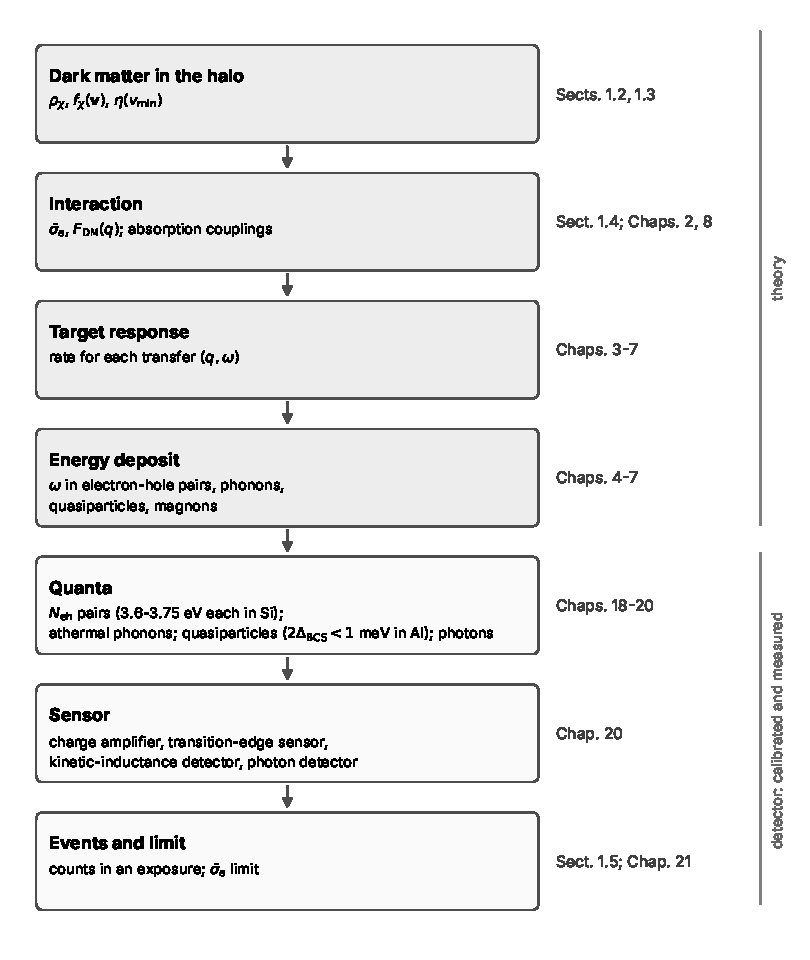
\includegraphics[width=0.78\linewidth]{figures/ch01/fig1_8.pdf}
  \caption{The signal chain from dark matter to sensor. The upper four steps are computed from theory: the halo (\cref{sec:1.2,sec:1.3}), the interaction (\cref{sec:1.4}; \cref{chap:2,chap:8}), the target response and the primary excitations (\cref{chap:3,chap:4,chap:5,chap:6,chap:7}). The lower three are fixed by calibration and measurement: the conversion of the deposit into countable quanta (\cref{chap:18,chap:20}), the sensor (\cref{chap:20}) and the statistical step from counts to a limit (\cref{sec:1.5}; \cref{chap:21}). Energies per quantum are from Refs.~\cites[Table~I]{ramanathan2020ionization}[Sect.~2.2.1]{hochberg2016detecting}.}
  \label{fig:1-chain}
\end{figure}

\subsection{Readout quanta}\label{sec:1.5-quanta}

A deposit of a few eV or less does not stay in the excitation that the dark matter created. Hot electrons and holes lose energy to further electron--hole pairs and to phonons; quasiparticles in a superconductor emit phonons; phonons decay into lower-energy phonons. Detectors read the products at one of four stages: as charge, as heat carried by phonons, as quasiparticles of a superconductor, or as photons~\cite[Sect.~VII]{kahn2022searches}. Each channel counts a different quantum, and the energy per quantum sets how finely a deposit is resolved.

\paragraph{Charge.} In a semiconductor an excitation across the band gap promotes an electron to the conduction band and leaves a vacancy, a \emph{hole}, in the valence band. The pair is called an \emph{electron--hole pair}. Both carriers are mobile, and an applied electric field drifts them to electrodes before they recombine~\cite[Sect.~VII\,A]{kahn2022searches}. The number of pairs produced by a deposit $\omega$ is the \emph{ionization yield} $N_{\mathrm{eh}}$. A primary carrier with energy well above the gap creates further pairs by impact ionization, knocking further electrons across the gap, and also emits phonons; on average, then, each pair costs more than $\Eg$. For deposits well above \SI{20}{eV} the mean yield is proportional to the deposit~\cite[abstract and Eq.~(1)]{ramanathan2020ionization},
\begin{equation}
  \langle N_{\mathrm{eh}}\rangle = \frac{\omega}{\varepsilon_{\mathrm{eh}}} ,
  \label{eq:1.5-yield}
\end{equation}
with the mean energy per pair $\varepsilon_{\mathrm{eh}}$. Measurements in silicon give \SIrange{3.62}{3.66}{eV} at \SI{300}{K} and \SIrange{3.70}{3.75}{eV} between \SI{5}{K} and \SI{123}{K}~\cite[Table~I]{ramanathan2020ionization}, roughly three times the gap. The excess goes into phonons. The fluctuations of $N_{\mathrm{eh}}$ are smaller than Poisson fluctuations: the variance is 0.1 to 0.15 times the mean~\cite[Eq.~(5.4)]{essig2016direct}. A \SI{100}{eV} deposit produces on average $100/3.7 = 27$ pairs with a spread of $(0.12 \times 27)^{1/2} = 1.8$, against $27^{1/2} = 5.2$ for a Poisson count. The pairs are not produced independently: the energy is fixed, and a cascade that makes one more pair has less energy left for the next.

Light dark matter, however, deposits only a few eV, where \cref{eq:1.5-yield} fails. Below $2\Eg$ energy conservation allows one pair at most; between that and a few tens of eV the yield depends on how the primary carriers share the energy, and the silicon data cover 3 to \SI{8}{eV} and then \SI{50}{eV} upward, with nothing in between~\cite[Sect.~III]{ramanathan2020ionization}. A widely used step model assigns one pair for the first $\Eg$ and one more for each further $\varepsilon_{\mathrm{eh}}$~\cite[Eq.~(5.1)]{essig2016direct},
\begin{equation}
  N_{\mathrm{eh}}(\omega) = 1 + \left\lfloor \frac{\omega - \Eg}{\varepsilon_{\mathrm{eh}}} \right\rfloor \qquad (\omega \ge \Eg),
  \label{eq:1.5-step}
\end{equation}
where $\lfloor x\rfloor$ is the largest integer not above $x$. With the low-temperature gap $\Eg = \SI{1.17}{eV}$ of \cref{we:1-mmin} and $\varepsilon_{\mathrm{eh}} = \SI{3.6}{eV}$~\cite[Eq.~(5.2)]{essig2016direct}, a \SI{5}{eV} deposit makes $1 + \lfloor 1.06\rfloor = 2$ pairs and a \SI{10}{eV} deposit $1 + \lfloor 2.45\rfloor = 3$. \Cref{chap:18} derives the yield from the carrier cascade.

A detector that counts pairs states its threshold as a number of pairs, and \cref{eq:1.5-step} turns that number into an energy. The $n$-th pair appears at $\omega = \Eg + (n-1)\varepsilon_{\mathrm{eh}}$, and thresholds of one, two and three pairs then correspond to 1.17, 4.77 and \SI{8.37}{eV}. Through $m_{\mathrm{min}} = 2E_{\mathrm{th}}/v_{\mathrm{max}}^2$ (\cref{eq:1.3-mmin}) with $v_{\mathrm{max}} = \num{2.650e-3}$, these translate into threshold masses of 0.33, 1.36 and \SI{2.38}{MeV}. A search that discards the single-pair bin, where the dark counts described below accumulate, gives up a factor of four in mass reach for a cleaner sample. Since the yield has not been measured in silicon between 8 and \SI{50}{eV}, the energy assigned to a three-pair threshold, and with it $m_{\mathrm{min}}$, carries a model uncertainty (\cref{sec:1.3-edge}).

Skipper charge-coupled devices and calorimetric detectors count single charges. A skipper charge-coupled device measures the charge in each pixel many times without destroying it; the noise falls with the square root of the number of measurements, below 0.1 electron per pixel~\cite[Sect.~VII\,A]{kahn2022searches}. A calorimetric detector instead drifts the carriers across a bias voltage $V_{\mathrm{bias}}$. Each carrier then emits phonons in proportion to the work done on it (the Neganov--Trofimov--Luke effect). The phonon energy is~\cite[Eq.~(195)]{kahn2022searches}
\begin{equation}
  E_{\mathrm{ph}} = E_{\mathrm{prim}} + N_{\mathrm{eh}}\, e V_{\mathrm{bias}} ,
  \label{eq:1.5-luke}
\end{equation}
where $E_{\mathrm{prim}}$ is the part of the deposit that went directly into phonons, at most $\omega$; the second term is usually much larger.
At $V_{\mathrm{bias}} = \SI{150}{V}$ each pair adds \SI{150}{eV}, and the spectrum shows peaks at integer $N_{\mathrm{eh}}$~\cite[Sect.~VII\,A]{kahn2022searches}. In both devices the lowest bins are polluted by a dark rate, charge that leaks across the gap without any deposit, and single-pair events carry the largest background.

\paragraph{Phonons.} Every excitation of a solid ends as phonons, the quantized lattice vibrations of \cref{sec:1.3}. A calorimeter measures this heat and with it the total deposit, whatever the primary excitation~\cite[Sect.~VII\,B]{kahn2022searches}. The phonons first created in silicon are optical phonons of about \SI{64}{meV}; through several anharmonic decays they eventually become acoustic phonons of a few meV. At an operating temperature of \SI{15}{mK} the thermal phonons carry about \SI{1}{\micro eV}, and the signal phonons are far from equilibrium (\emph{athermal}) and cross the crystal ballistically before they reach a sensor on the surface~\cite[Sect.~VII\,B]{kahn2022searches}. The quanta are too numerous and too soft to count one by one. The sensor integrates their energy, and its noise sets the threshold: a \SI{10.6}{g} silicon crystal read by a tungsten transition-edge sensor reaches a resolution of \SI{3.86}{eV} and a threshold of \SI{16.3}{eV}~\cite[Sect.~VII\,B]{kahn2022searches}. A transition-edge sensor is a superconducting film held at the edge of its transition, where a small heat input produces a large change in resistance. Phonons are treated precisely in \cref{sec:5.3}.

\paragraph{Quasiparticles.} In a superconductor the electrons near the Fermi level, the energy that separates occupied from empty states, bind into Cooper pairs. Breaking a pair costs $2\Delta_{\mathrm{BCS}}$, where $\Delta_{\mathrm{BCS}}$ is the superconducting gap, and creates two \emph{quasiparticles}, the excitations of the paired state (made precise in \cref{sec:7.2}). The Bardeen--Cooper--Schrieffer (BCS) theory relates the gap to the critical temperature, $\Delta_{\mathrm{BCS}} \approx 1.76\,k_{\mathrm{B}}T_{\mathrm{c}}$~\cite[Sect.~3.3]{essig2022snowmass}. With $T_{\mathrm{c}} = \SI{1.2}{K}$ for bulk aluminum~\cite{yeh2023doubling}, $2\Delta_{\mathrm{BCS}} \approx \SI{0.36}{meV}$. Thin films have higher critical temperatures~\cite{yeh2023doubling}, and dark-matter projections adopt the film value $2\Delta_{\mathrm{BCS}} = \SI{0.6}{meV}$~\cites[Sect.~2.2.1]{hochberg2016detecting}[Table~II]{mitridate2021dark}. A deposit in a superconducting absorber cascades through quasiparticles and phonons until no phonon can break another pair; about \SI{60}{\percent} of the energy ends as quasiparticles and the rest as phonons near $2\Delta_{\mathrm{BCS}}$~\cite[Sect.~2.2.1]{hochberg2016detecting}. Quasiparticles also convert phonons into a signal. In transition-edge sensors and in kinetic-inductance detectors, superconducting resonators whose frequency shifts when pairs are broken, phonons from the crystal break Cooper pairs in a superconducting film, and the change in the film's resistance or impedance is read out~\cite[Sect.~3.3.1]{essig2022snowmass}. The pair-breaking energy is the smallest quantum in \cref{tab:1-quanta}. If a single broken pair in an aluminum absorber could be detected, \cref{eq:1.3-mmin} with the bulk value $E_{\mathrm{th}} = \SI{0.36}{meV}$ would place the threshold mass at \SI{0.10}{keV} (\SI{0.17}{keV} for the film value), below the keV lower end of the window of \cref{sec:1.1}. Present sensors are far from this: their thresholds are set by noise, not by the quantum.

\paragraph{Photons.} A scintillator returns part of the deposit as photons. In NaI and CsI, with band gaps of about \SI{6}{eV}, these are optical or near-ultraviolet photons of a few eV; GaAs, with its gap of \SI{1.52}{eV}, emits in the infrared~\cite[Sect.~VII\,C]{kahn2022searches}. The photons are counted by a photomultiplier, by a transition-edge sensor or by a silicon device, in which each photon above the silicon gap, \SI{1.17}{eV} at low temperature (\cref{we:1-mmin}), creates electron--hole pairs.

\Cref{tab:1-quanta} collects the four channels: charge, phonons, quasiparticles and photons. In every case the detector sees a number of quanta, or their summed energy, after the cascade. The relation between that number and $\omega$ is an input to every limit, and for deposits of a few eV it is the most poorly known step of the chain.

\begin{table}[tbp]
  \caption{Readout channels, the quantum each counts and its energy in silicon or aluminum, with the sensors that read them. The phonon and quasiparticle energies set the scale of the quanta; calorimetric sensors integrate many of them.}
  \label{tab:1-quanta}
  \centering\small
  \begin{tabular}{@{}>{\raggedright\arraybackslash}p{0.16\linewidth}>{\raggedright\arraybackslash}p{0.19\linewidth}>{\raggedright\arraybackslash}p{0.29\linewidth}>{\raggedright\arraybackslash}p{0.27\linewidth}@{}}
    \toprule
    Channel & Quantum & Energy per quantum & Sensor \\
    \midrule
    Charge & electron--hole pair & $\varepsilon_{\mathrm{eh}} = 3.6$ to \SI{3.75}{eV} in Si (at least $\Eg$ for the first pair) & skipper charge-coupled device (CCD); phonon calorimeter with bias \\
    Heat & athermal phonon & \SI{60}{meV} optical at creation, a few meV after decay, in Si & transition-edge sensor \\
    Quasiparticles & broken Cooper pair & $2\Delta_{\mathrm{BCS}} \approx \SI{0.36}{meV}$ in bulk Al & transition-edge sensor; kinetic-inductance detector \\
    Light & photon & a few eV (optical, near-ultraviolet); infrared in GaAs & photomultiplier; transition-edge sensor; Si photodetector \\
    \bottomrule
  \end{tabular}
\end{table}

\subsection{Event rate}\label{sec:1.5-rate}

The event rate $\mathcal{R}$ of \cref{eq:1.1-rate}, the expected number of events per unit time per unit target mass, is quoted in \si{kg^{-1}.yr^{-1}}. Its \emph{spectrum} $\dd\mathcal{R}/\dd\omega$ is the rate per unit deposited energy, and $\mathcal{R}$ is the integral of the spectrum above the threshold $E_{\mathrm{th}}$ (\cref{sec:1.3}). A detector of mass $M_{\mathrm{det}}$ that runs for a live time $t_{\mathrm{exp}}$ collects the \emph{exposure} $M_{\mathrm{det}}t_{\mathrm{exp}}$, quoted in kg\,yr. The expected number of signal events is
\begin{equation}
  N_{\mathrm{sig}} = M_{\mathrm{det}}\,t_{\mathrm{exp}}\,\mathcal{R} ,
  \label{eq:1.5-Nsig}
\end{equation}
where $\mathcal{R}$ includes the probability that an event passes the selection. The absorption rate of \cref{eq:1.4-dp-abs} uses the same normalization per unit target mass.

A charge detector does not measure $\omega$ but $N_{\mathrm{eh}}$. The rate of events with $n$ pairs collects the spectrum over the deposits that \cref{eq:1.5-step} maps to $n$,
\begin{equation}
  \mathcal{R}_n = \int_{\Eg + (n-1)\varepsilon_{\mathrm{eh}}}^{\Eg + n\varepsilon_{\mathrm{eh}}}\dd\omega\,\frac{\dd\mathcal{R}}{\dd\omega} ,
  \label{eq:1.5-bins}
\end{equation}
and a search compares the counts in each bin with the expected background in that bin. Since for scattering through a heavy mediator in silicon the typical deposit is a few eV, the spectrum peaks in the two-pair bin~\cite[Fig.~7]{essig2016direct}.

The schematic rate of \cref{eq:1.1-rate} becomes concrete for a target whose response depends on the magnitude $q$ of the momentum transfer but not on its direction, as for a liquid, an atom or a crystal averaged over orientations. The velocity integral and the average over the direction of $\vect{q}$ then act on the delta function alone, and \cref{sec:1.3-eta} turned them into the measure $q\,\dd q\,\eta(\vmin)/4\pi^2$. With the coupling of \cref{eq:1.4-Vsq} and the halo of \cref{sec:1.2}, the factors of \cref{sec:1.1} combine into~\cite[Eq.~(11)]{kahn2022searches}
\begin{equation}
  \mathcal{R} = \frac{1}{\rho_T}\,\underbrace{\frac{\rho_\chi}{m_\chi}}_{\text{halo}}\int\frac{q\,\dd q}{(2\pi)^2}\int\dd\omega\;\underbrace{\eta\bigl(\vmin(q,\omega)\bigr)}_{\text{halo, kinematics}}\,\underbrace{\frac{\pi\sigmae\FDM(q)^2}{\mu_{\chi e}^2}}_{\text{coupling}}\,\underbrace{S(q,\omega)}_{\text{target}}.
  \label{eq:1.5-rate}
\end{equation}
\Cref{sec:2.5} derives it term by term from the thermal golden rule, and \cref{sec:4.2} develops the properties of $S(q,\omega)$. Here we read off how $\mathcal{R}$ depends on the dark-matter parameters.

For a crystal, $S(q,\omega)$ is computed from the electronic states of the material. Density-functional theory supplies the bands and wavefunctions as Kohn--Sham states, the eigenstates of an effective one-electron problem rather than of the interacting electrons. Their overlaps at momentum transfer $q$, the crystal form factors, fix the transition probabilities; \cref{app:E.7} describes how these are evaluated and converged, and \cref{app:E.6} adds screening. This step is where most of the theory uncertainty of a limit originates.

Define the response-weighted average of the squared form factor,
\begin{equation}
  \langle\FDM^2\rangle = \frac{\int q\,\dd q\int\dd\omega\;\eta(\vmin)\,S(q,\omega)\,\FDM(q)^2}{\int q\,\dd q\int\dd\omega\;\eta(\vmin)\,S(q,\omega)} ,
  \label{eq:1.5-FDMavg}
\end{equation}
which is 1 for a heavy mediator and $\langle(q_0/q)^4\rangle$ for a light one. Then \cref{eq:1.5-rate} reads
\begin{equation}
  \mathcal{R} = \frac{\pi\sigmae\,\rho_\chi\,\langle\FDM^2\rangle}{\rho_T\, m_\chi\,\mu_{\chi e}^2}\int\frac{q\,\dd q}{(2\pi)^2}\int\dd\omega\;\eta(\vmin)\,S(q,\omega) .
  \label{eq:1.5-scaling}
\end{equation}
We see that the rate is linear in $\sigmae$ and in $\rho_\chi$, and $\sigmae$ appears nowhere else. The mass enters through the number density, the reduced mass and the region of the last integral. The number density brings $1/m_\chi$. The reduced mass tends to $m_e$ once $m_\chi \gg m_e$, and the factor $\mu_{\chi e}^2$ stops changing above a few MeV. The last integral depends on $m_\chi$ only through the momentum transfers allowed by $\vmin(q,\omega) \le v_{\mathrm{max}}$ (\cref{eq:1.3-region}): it vanishes for $m_\chi \le m_{\mathrm{min}}$ and stops growing once $2m_\chi v_{\mathrm{max}}$ exceeds the momenta at which $S(q,\omega)$ is appreciable. Well above threshold, then,
\begin{equation}
  \mathcal{R} \propto \frac{\sigmae\,\rho_\chi\,\langle\FDM^2\rangle}{m_\chi} .
  \label{eq:1.5-heuristic}
\end{equation}
This is a statement about scaling only; the absolute rate needs $S(q,\omega)$ and the full integral. As a check of \cref{eq:1.5-rate}, in natural units $\rho_\chi/(\rho_T m_\chi)$ has dimension $\mathrm{eV}^{-1}$ (an inverse mass), $q\,\dd q\,\dd\omega$ has $\mathrm{eV}^3$, $\sigmae/\mu_{\chi e}^2$ has $\mathrm{eV}^{-4}$, $S(q,\omega)$ has $\mathrm{eV}^2$ with the normalization of \cref{sec:4.2}, and $\eta$, an inverse speed, is dimensionless. The product is dimensionless, as a rate (eV) per unit mass (eV) must be.

\subsection{Counting and the upper limit}\label{sec:1.5-limit}

Since dark-matter events are rare and independent, their number in a fixed exposure follows the Poisson distribution. To see this, divide the exposure into $K$ equal parts, each so small that it holds one event with probability $p = N_{\mathrm{sig}}/K$ and two events with negligible probability. The probability of $N_{\mathrm{obs}}$ events is binomial,
\begin{equation*}
  \binom{K}{N_{\mathrm{obs}}} p^{N_{\mathrm{obs}}}(1-p)^{K-N_{\mathrm{obs}}}
  = \frac{K(K-1)\cdots(K-N_{\mathrm{obs}}+1)}{K^{N_{\mathrm{obs}}}}\,\frac{N_{\mathrm{sig}}^{N_{\mathrm{obs}}}}{N_{\mathrm{obs}}!}\left(1-\frac{N_{\mathrm{sig}}}{K}\right)^{K-N_{\mathrm{obs}}} .
\end{equation*}
As $K \to \infty$ at fixed $N_{\mathrm{obs}}$, the first fraction tends to 1 and the last factor to $\ee^{-N_{\mathrm{sig}}}$, and we are left with
\begin{equation}
  P(N_{\mathrm{obs}}\,|\,N_{\mathrm{sig}}) = \frac{N_{\mathrm{sig}}^{N_{\mathrm{obs}}}}{N_{\mathrm{obs}}!}\,\ee^{-N_{\mathrm{sig}}} .
  \label{eq:1.5-poisson}
\end{equation}

Suppose a search sees no events and expects no background. A large $N_{\mathrm{sig}}$ would make this outcome improbable, since $P(0\,|\,N_{\mathrm{sig}}) = \ee^{-N_{\mathrm{sig}}}$. The upper limit at \SI{90}{\percent} confidence, $N_{90}$, is the expected count at which the observed outcome, or one with fewer events, would occur in only \SI{10}{\percent} of repeated experiments. Every larger $N_{\mathrm{sig}}$ would yield at least one event more than \SI{90}{\percent} of the time, and is excluded at that confidence. The confidence level describes the procedure, not the parameter: if the experiment were repeated many times and the limit computed the same way each time, the interval from 0 to $N_{90}$ would contain the true $N_{\mathrm{sig}}$ in at least \SI{90}{\percent} of the repetitions. It is not the probability that $\sigmae$ lies below the limit, which would require a prior distribution for $\sigmae$. Setting $\ee^{-N_{90}} = 0.1$ gives
\begin{equation}
  N_{90} = \ln 10 = 2.303 .
  \label{eq:1.5-N90}
\end{equation}
At \SI{95}{\percent} confidence the same condition leads to $\ln 20 = 3.00$, the three events assumed in many projections~\cite[Sect.~V]{mitridate2021dark}. If instead $N_{\mathrm{obs}}$ events are seen and all are kept as possible signal, the \SI{90}{\percent} limit solves $\sum_{n=0}^{N_{\mathrm{obs}}} P(n\,|\,N_{90}) = 0.1$. A numerical solution yields $N_{90} = 3.89$ for one event and 5.32 for two. Such a limit holds whatever the origin of the observed events.

Since $\mathcal{R}$ is proportional to $\sigmae$ (\cref{eq:1.5-scaling}), we write $\mathcal{R} = \sigmae\,r(m_\chi)$ with $r(m_\chi)$ the rate per unit cross-section. Setting $N_{\mathrm{sig}} = N_{90}$ in \cref{eq:1.5-Nsig} gives the limit:

\begin{keyresult}[Zero-background limit]
A search with exposure $M_{\mathrm{det}}t_{\mathrm{exp}}$ that observes no events and expects no background excludes at \SI{90}{\percent} confidence
\begin{equation}
  \sigmae > \sigmae^{\mathrm{lim}}(m_\chi) = \frac{N_{90}}{M_{\mathrm{det}}\,t_{\mathrm{exp}}\; r(m_\chi)}, \qquad N_{90} = 2.303 .
  \label{eq:1.5-limit}
\end{equation}
The limit improves in proportion to the exposure, $\sigmae^{\mathrm{lim}} \propto 1/(M_{\mathrm{det}}t_{\mathrm{exp}})$.
\end{keyresult}

Background changes the scaling. Suppose the background is known to give $N_{\mathrm{bkg}} = \mathcal{R}_{\mathrm{bkg}}\,M_{\mathrm{det}}t_{\mathrm{exp}}$ events, with $\mathcal{R}_{\mathrm{bkg}}$ the background rate per unit exposure, and cannot be removed event by event. The observed count then fluctuates by roughly $N_{\mathrm{bkg}}^{1/2}$, and a signal is excluded only when it exceeds a fixed multiple $k$ of that fluctuation, $\sigmae\,r\,M_{\mathrm{det}}t_{\mathrm{exp}} \ge k\,(\mathcal{R}_{\mathrm{bkg}}\,M_{\mathrm{det}}t_{\mathrm{exp}})^{1/2}$. Solving for $\sigmae$, we find $\sigmae^{\mathrm{lim}} = k\,\mathcal{R}_{\mathrm{bkg}}^{1/2}/[r\,(M_{\mathrm{det}}t_{\mathrm{exp}})^{1/2}]$: the limit now improves only as the inverse square root of the exposure.

Counting alone cannot tell signal from background, but the annual modulation of \cref{sec:1.2} can. For momentum transfers that need $\vmin = \SI{600}{km.s^{-1}}$, $\eta$ is \SI{21}{\percent} above its reference value in June and \SI{16}{\percent} below it in December (\cref{sec:1.2}). Take the modulation as a cosine with amplitude $A_{\mathrm{mod}} = 0.185$, the mean of the two. Averaged over the half-year centered on June, a cosine of amplitude $A_{\mathrm{mod}}$ has mean $2A_{\mathrm{mod}}/\pi = 0.118$; with $N$ events expected per half-year, the June half then exceeds the December half by $2 \times 0.118\,N = 0.236\,N$. The Poisson fluctuation of the difference of two counts of about $N$ each is $(2N)^{1/2}$. A difference of two standard deviations requires $0.236\,N \ge 2(2N)^{1/2}$, that is $N \ge 144$ events per half-year. A modulation test needs a detected signal of a few hundred events, far beyond the few events that set a limit. \Cref{chap:21} treats the statistics in full.

\begin{workedexample}{Expected events and a limit for a toy rate}\label{we:1-limit}
We take a silicon target, $m_\chi = \SI{100}{MeV}$, a heavy mediator and $\rho_\chi = \SI{0.3}{GeV.cm^{-3}}$. For the toy rate we keep the prefactor of the silicon rate of Ref.~\cite[Eq.~(3.13)]{essig2016direct}. That equation is written for the spectrum per unit logarithm of the deposit, $\dd\mathcal{R}/\dd\ln\omega$, and the reference describes its remaining integral as roughly unity for typical $q$ and $\omega$. We set that integral equal to one between $\Eg = \SI{1.17}{eV}$ and \SI{30}{eV}, the range of the toy response of \cref{fig:1-exclusion}, and to zero elsewhere. Integrating over $\ln\omega$ then multiplies the prefactor by $\ln(30/1.17) = 3.24$, and the toy rate is
\begin{equation*}
  \mathcal{R}_{\mathrm{toy}} = \ln\!\left(\frac{\SI{30}{eV}}{\Eg}\right)\frac{\rho_\chi}{m_\chi}\,\frac{\sigmae}{M_{\mathrm{cell}}}\,\alpha\,\frac{m_e^2}{\mu_{\chi e}^2} .
\end{equation*}
Here $M_{\mathrm{cell}} = \SI{52.33}{GeV}$ is the mass of the two-atom silicon unit cell~\cite[below Eq.~(3.13)]{essig2016direct}, so $1/M_{\mathrm{cell}}$ is the number of cells per unit mass. The factor $\alpha = q_0/m_e$ is the typical speed of a bound electron, $\alpha c$ in conventional units. The factors are:
$\rho_\chi/m_\chi = \SI{3}{cm^{-3}}$;
$\SI{1}{kg} = \SI{5.610e26}{GeV}$, so a kilogram holds $\num{1.072e25}$ cells;
$\alpha c = \SI{2.188e8}{cm.s^{-1}}$;
$\mu_{\chi e} = \SI{0.5084}{MeV}$, so $m_e^2/\mu_{\chi e}^2 = 1.010$.
Without the logarithm their product is \SI{7.106e33}{cm^{-2}.s^{-1}.kg^{-1}}; with it, $\mathcal{R}_{\mathrm{toy}}/\sigmae = \SI{2.305e34}{cm^{-2}.s^{-1}.kg^{-1}}$. With $\SI{1}{yr} = \SI{3.156e7}{s}$ this is $r = \SI{7.28e41}{cm^{-2}.kg^{-1}.yr^{-1}}$.
For an exposure of \SI{1}{kg.yr} and $\sigmae = \SI{e-40}{cm^2}$, \cref{eq:1.5-Nsig} predicts $N_{\mathrm{sig}} = 73$ events. With no events observed, \cref{eq:1.5-limit} gives
\begin{equation*}
  \sigmae^{\mathrm{lim}} = \frac{2.303}{(\SI{1}{kg.yr})(\SI{7.28e41}{cm^{-2}.kg^{-1}.yr^{-1}})} = \SI{3.2e-42}{cm^2},
\end{equation*}
and ten times the exposure brings it to \SI{3.2e-43}{cm^2}. Since the toy has no material response and no yield model, these numbers show only the arithmetic and the scaling; a real silicon search must compute $S(q,\omega)$ and fold in \cref{eq:1.5-step} and the efficiency.
\end{workedexample}

\subsection{Exclusion plots}\label{sec:1.5-plot}

Results of light-dark-matter searches are shown as \emph{exclusion limits}: the curve $\sigmae^{\mathrm{lim}}(m_\chi)$ of \cref{eq:1.5-limit} in the plane of $m_\chi$ and $\sigmae$, drawn separately for a heavy and a light mediator. Every point above the curve would have produced more than $N_{90}$ events and is excluded. By \cref{eq:1.5-limit,eq:1.5-scaling},
\begin{equation}
  \sigmae^{\mathrm{lim}}(m_\chi) \propto \frac{m_\chi\,\mu_{\chi e}^2}{\rho_\chi\,\langle\FDM^2\rangle\,M_{\mathrm{det}}t_{\mathrm{exp}}}\left[\int\frac{q\,\dd q}{(2\pi)^2}\int\dd\omega\;\eta(\vmin)\,S(q,\omega)\right]^{-1},
  \label{eq:1.5-limscaling}
\end{equation}
and the shape of the curve follows from the mass dependence discussed after \cref{eq:1.5-scaling}. \Cref{fig:1-exclusion} shows the shapes for a toy response; \cref{chap:21} treats real limits.

\begin{figure}[tbp]
  \centering
  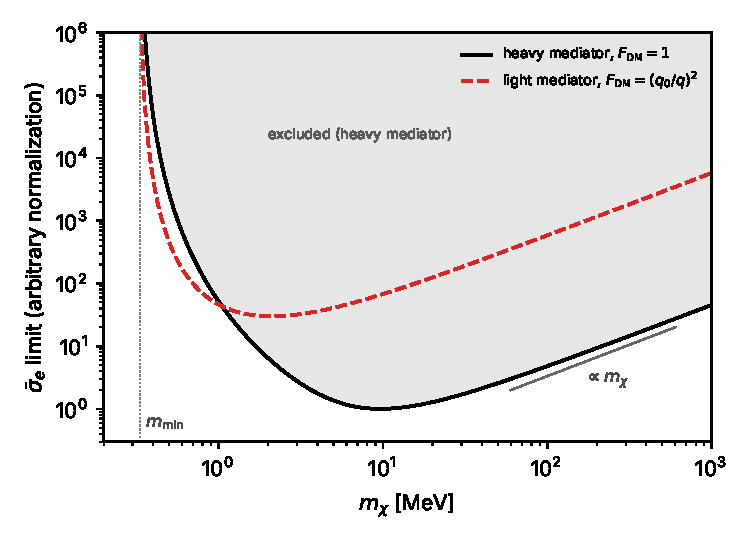
\includegraphics[width=0.72\linewidth]{figures/ch01/fig1_9.pdf}
  \caption{Schematic exclusion limits on $\sigmae$ for a silicon-like target. The threshold is the low-temperature gap $\Eg = \SI{1.17}{eV}$. The curves follow from \cref{eq:1.5-limscaling} with the standard-halo $\eta(\vmin)$ of \cref{sec:1.3} and a toy response: $S(q,\omega)$ flat between $\Eg$ and \SI{30}{eV}, multiplied by the Gaussian cutoff $\exp[-q^2/2(2q_0)^2]$ with $q_0 = \alpha m_e = \SI{3.73}{keV}$. Each curve has an arbitrary normalization (the light-mediator curve is shifted up for legibility). Both curves rise without bound at the threshold mass $m_{\mathrm{min}} = \SI{0.33}{MeV}$ (dotted) and grow as $m_\chi$ at large mass. The heavy-mediator curve ($\FDM = 1$) reaches its minimum at \SI{9.7}{MeV}, where the allowed momenta cover the cutoff; the light-mediator curve ($\FDM = (q_0/q)^2$), dominated by the smallest $q$, reaches its minimum at \SI{2.1}{MeV}. The shaded region is excluded by the heavy-mediator search.}
  \label{fig:1-exclusion}
\end{figure}

\paragraph{The low-mass edge.} Below $m_{\mathrm{min}} = 2E_{\mathrm{th}}/v_{\mathrm{max}}^2$ (\cref{eq:1.3-mmin}) no dark-matter particle in the halo can deposit $E_{\mathrm{th}}$, the integral in \cref{eq:1.5-limscaling} vanishes and the limit is infinite. Just above $m_{\mathrm{min}}$ only the fastest particles contribute, and $\eta$ grows from zero quadratically in the distance from the escape speed (\cref{eq:1.3-edge}): the curve falls steeply from a vertical wall. The position of the wall depends only on the threshold and on $v_{\mathrm{max}}$; a lower threshold moves it to lower mass in proportion (\cref{sec:1.3-edge}).

\paragraph{The heavy-mediator slope.} With $\FDM = 1$ the integrand of \cref{eq:1.5-limscaling} grows with $q$ through the factor $q\,\dd q$, and the maximum momentum transfer, $2m_\chi v_{\mathrm{max}}$, grows with $m_\chi$. It equals $q_0$ at \SI{0.70}{MeV} (\cref{sec:1.3}). The integral keeps growing until $2m_\chi v_{\mathrm{max}}$ passes the momenta of the valence electrons, a few $q_0$, which happens at masses around \SI{10}{MeV}; the curve falls over this whole range. Above it the integral is constant, $\mu_{\chi e} = m_e$, and only the factor $m_\chi$ remains: $\sigmae^{\mathrm{lim}} \propto m_\chi$, a line of slope one on logarithmic axes. The heavier dark matter is less numerous at fixed $\rho_\chi$.

\paragraph{The light-mediator slope.} With $\FDM = (q_0/q)^2$ the weight $(q_0/q)^4\,q\,\dd q$ favors the smallest momentum transfer that can deposit the threshold, $q \approx E_{\mathrm{th}}/v_{\mathrm{max}}$ (\cref{sec:1.3}). That momentum transfer is reachable as soon as $m_\chi$ is a few times $m_{\mathrm{min}}$, and the light-mediator curve turns over close to the edge, growing as $m_\chi$ from a few MeV upward. Because the rate comes from small $q$, the light-mediator limit is also the one most affected by screening (\cref{sec:4.4}) and by the low-energy end of the ionization yield.

As a result, the two curves are not related by a constant factor, and a limit quoted for one mediator cannot be rescaled to the other without the response. In the toy of \cref{fig:1-exclusion} the heavy-mediator limit at \SI{1}{MeV} stands a factor of 49 above its minimum at \SI{9.7}{MeV}, while the light-mediator limit is already within a factor of 1.5 of its minimum at \SI{2.1}{MeV}. A two-pair threshold would move both walls from 0.33 to \SI{1.36}{MeV}. Real exclusion plots add curves from several experiments and the benchmark cross-sections of thermal and freeze-in models (\cref{we:1-darkphoton}).

\subsection{Inputs of a limit}\label{sec:1.5-inputs}

Every exclusion curve combines measured inputs from the detector with theory inputs, and \cref{fig:1-chain} marks the boundary. The measured inputs belong to the detector: the exposure $M_{\mathrm{det}}t_{\mathrm{exp}}$, the threshold, the efficiency with which events pass the selection, the background and the observed count. Their errors are statistical or come from calibration, and experiments propagate them.

The theory inputs are the halo parameters, the particle-physics model and the response of the target. The halo parameters $\rho_\chi$, $v_0$ and $v_{\mathrm{esc}}$ are fixed by convention to the values of \cref{sec:1.2} so that experiments can be compared (\cref{app:A.8}); the limit scales as $1/\rho_\chi$, and $v_{\mathrm{esc}}$ moves the edge (\cref{sec:1.3-edge}). The particle physics enters only through $\FDM$, which is a definition of the model rather than an approximation (\cref{sec:1.4}). The target enters through $S(q,\omega)$ and through the conversion from $\omega$ to quanta, $N_{\mathrm{eh}}(\omega)$ for charge detectors. Both are computed, not measured, in the eV range that matters for light dark matter. Their errors are not statistical: they come from approximations, such as the treatment of exchange and correlation in the band structure, the neglect of screening or of phonons, or the step model of \cref{eq:1.5-step}. A longer exposure does not reduce them. Their effect on a limit follows from \cref{eq:1.5-limscaling}. A fractional error in $S(q,\omega)$ at the momentum transfers that dominate the integral moves the limit by the same fraction. An error in the gap or in the threshold energy moves the edge, $\delta\ln m_{\mathrm{min}} = \delta\ln E_{\mathrm{th}}$ (\cref{sec:1.3-edge}), and near the edge it changes the limit by a much larger factor, because $\eta$ varies steeply there. Together these errors make up the \emph{theory uncertainty} of a limit.

Two lines of argument start here: the signal chain and the theory uncertainty. The first follows the signal chain of \cref{fig:1-chain} from the response of the target to the measured signal: \crefrange{chap:2}{chap:7} build the response, and later chapters follow the deposit through the cascade to the sensor (\cref{chap:18,chap:20}). The second follows the theory uncertainty: each approximation, when it is introduced, comes with an estimate of its error, and \cref{chap:21} turns these estimates into uncertainties on exclusion limits.

\section*{Summary}

The event rate is an integral over a product of three factors, the halo, the coupling $|\tilde V(\vect q)|^2$ and the dynamic structure factor $S(\vect q,\omega)$ of the target, tied together by energy conservation (\cref{sec:1.1}). The particle physics and the condensed-matter physics therefore separate, and most of the book computes $S$. Gravity measures the density of dark matter but not its mass: a local density of a few tenths of a \si{GeV.cm^{-3}} (\cref{sec:1.2}) and a cosmological density $\Omega_{\mathrm{c}}h^2 = 0.120$ from the cosmic microwave background. The mass is open over some 90 decades, and the keV--GeV window is the range where the kinetic energy of halo dark matter, $\frac12 m_\chi v^2$ with $v \approx 10^{-3}$, matches the meV--eV excitations of solids. A thermal relic needs $\langle\sigma v\rangle \approx \SIrange{2e-26}{3e-26}{cm^3.s^{-1}}$, which below a few GeV requires a light mediator; freeze-in is the main alternative.

The local halo is described by the standard halo model (\cref{sec:1.2}): a truncated Maxwell--Boltzmann distribution with $\rho_\chi = \SI{0.3}{GeV.cm^{-3}}$, $v_0 = \SI{238}{km.s^{-1}}$ and $v_{\mathrm{esc}} = \SI{544}{km.s^{-1}}$, seen in the laboratory through the Earth's motion. The largest laboratory speed is $v_{\mathrm{max}} = \SI{794.5}{km.s^{-1}}$. The Earth's orbit modulates the rate annually, with a phase that reverses at $\vmin \approx \SI{211}{km.s^{-1}}$, and its rotation turns a crystal through the dark-matter wind once per sidereal day.

Kinematics (\cref{sec:1.3}) relates the momentum $q$ and energy $\omega$ given to the target through $\omega_{\vect{q}} = \vect q\cdot\vect v - q^2/2m_\chi - \Delta_\chi$, and every scattering rate contains $\eta(\vmin)$, the mean inverse speed above the minimum speed $\vmin$. A threshold $E_{\mathrm{th}}$ is reachable only above $m_{\mathrm{min}} = 2E_{\mathrm{th}}/v_{\mathrm{max}}^2$, \SI{0.33}{MeV} for the low-temperature silicon gap. Near $m_{\mathrm{min}}$ the rate vanishes quadratically with the tail of the halo. Electron transitions involve momentum transfers comparable to $q_0 = \alpha m_e = \SI{3.73}{keV}$, close to the shortest reciprocal-lattice vector of silicon, and free nuclear recoils deposit little energy for sub-GeV dark matter.

A mediator of mass $m_V$ produces the potential $\tilde V(q) = y_\chi y_e/(q^2 + m_V^2)$ (\cref{sec:1.4}). Its strength is quoted as the vacuum reference cross-section $\sigmae$ and its momentum dependence as $\FDM(q)$, equal to 1 for a heavy and $(q_0/q)^2$ for a light mediator. The dark photon is the standard example; bosonic dark matter can instead be absorbed, depositing $\omega \approx m_\phi$ at $q \approx 0$.

A detector counts electron--hole pairs (\SIrange{3.6}{3.75}{eV} each in silicon), phonons, quasiparticles (about \SI{0.36}{meV} per pair in bulk aluminum) or photons (\cref{sec:1.5}). The rate is linear in $\sigmae$ and $\rho_\chi$ and falls as $1/m_\chi$ well above threshold. With no events and no background the \SI{90}{\percent} upper limit is 2.3 expected events, and the cross-section limit improves in proportion to the exposure. Exclusion curves have a vertical edge at $m_{\mathrm{min}}$ and grow as $m_\chi$ at large mass. Their accuracy rests on the computed response of the target, which \crefrange{chap:2}{chap:7} develop. The errors of that computation, the theory uncertainty, do not shrink with exposure, and the book estimates them with each approximation it makes.

\printbibliography[heading=subbibliography]
